\documentclass{ituthesis}

\settitle{Copatterns in Idris}
\setauthor{Sune Alk\ae rsig \& Thomas Hallier Didriksen}
\setsupervisor{Peter Sestoft}
\setextrasupervisor{David Christiansen}
\setdate{March 2015}

\usepackage[utf8]{inputenc}
\usepackage{url}
\usepackage{alltt}
\usepackage{amssymb, amsfonts, amsmath, amsthm}
\usepackage{listings}
\usepackage{natbib}
\usepackage{pdflscape}
\usepackage{todonotes}
\bibliographystyle{alpha}

\newcommand{\IdrisM}{Idris$^{-}$}
\newcommand{\later}{\rhd}
% Kappa commands
\newcommand{\onk}[1]{#1^\kappa}
\newcommand{\laterkappa}{\later^{\!\!\!\kappa}}
\newcommand{\laterk}[1]{\later^{\!\!\!\kappa}#1^\kappa}
\newcommand{\forallk}[1]{\forall\kappa.#1^\kappa}
\newcommand{\flaterk}[1]{\forall\kappa.\later^{\!\!\!\kappa}#1^\kappa}
% Kappa prime commands
\newcommand{\onkp}[1]{#1^\kappa'}
\newcommand{\laterkappap}{\later^{\!\!\!\kappa'}}
\newcommand{\laterkp}[1]{\later^{\!\!\!\kappa'}#1^{\kappa'}}
\newcommand{\forallkp}[1]{\forall\kappa'.#1^{\kappa'}}
\newcommand{\flaterkp}[1]{\forall\kappa'.\later^{\!\!\!\kappa'}#1^{\kappa'}}
\newcommand{\tensor}{\circledast}

% Theorem Styles
\newtheorem{theorem}{Theorem}[section]
\newtheorem{lemma}[theorem]{Lemma}
\newtheorem{proposition}[theorem]{Proposition}
\newtheorem{corollary}[theorem]{Corollary}
% Definition Styles
\theoremstyle{definition}
\newtheorem{definition}{Definition}[section]
\newtheorem{example}{Example}[section]
\theoremstyle{remark}
\newtheorem{remark}{Remark}

\begin{document}

\frontmatter

\thetitlepage
\newpage

\chapter*{Abstract}
This is an abstract

\cleardoublepage
\setcounter{tocdepth}{1}
\tableofcontents

\mainmatter
\midsloppy
\sloppybottom

%!TEX root = ../copatterns-thesis.tex
\chapter{Introduction}

%!TEX root = ../copatterns-thesis.tex
\chapter{Background}

% Sune
%#############
% Hvad er copatterns?
% Hvorfor giver copatterns mening, isoleret set?
% Hvor kommer copatterns fra? (Hagino, Abel og venner)
% Definition ved observation (eliminationsregler)
% Eksempler

% Ny viden: Copatterns
%#############

\section{Copatterns}
\label{sec:copatterns}
In functional programming, inductive data is commonly defined by \emph{constructors} in an
elegant and simple fashion. The data can be analyzed and manipulated using
pattern matching, which follows nicely from the finite nature of inductive
data. The growing consensus\todo{Among who?} is that coinductive data should be defined by
\emph{observations} due to its possible infinity. This\todo{Perhaps say this at
  the beginning?} means that one should distingush
between finite and infinite data. Hagino\todo{Hagino introduced a construct for
  synthesizing coinductive data. The distinction between finite and infinite
  data was already known.} first introduced this idea in his SymML
language \,\citep{Hagino89}, where the programmer could define coinductive types
by their \emph{destructors} or \emph{observations}. In other words\todo{We have
  to be precise here. }, inductive
types should be defined by their \emph{introduction rules}, and coinductive types by
their \emph{elimination rules}.

\begin{figure}[h]
\begin{lstlisting}[mathescape]
corecord Stream : Type -> Type where
  head : Stream a -> a
  tail : Stream a -> Stream a 
  constructor MkStream
\end{lstlisting}
\caption{An infinite list defined by observations.}
\label{fig:stream}
\end{figure}

The syntax for \texttt{codata} definitions presented in
Figure~\ref{fig:stream} defines a coinductive type by observations, as oppose to
by constructors. On a \texttt{Stream}, two observations can be made:
\texttt{head} and \texttt{tail}. The former provides us with the first element
of the stream, while the latter gives us with the rest of the infinite stream,
upon which another element can be observed with \texttt{head}. 

\emph{Destructor copatterns}, or simply
\emph{copatterns}\,\citep{Abel13Copatterns}, provide a way of defining functions
on coinductive data in terms of observations. Like pattern matching allows us to
define functions on inductive data by analyzing the structure of the input,
copatterns enable us to make experiments on functions with a result of
coinductive type.

The \texttt{Stream} defined by observations can be used to define a function
\texttt{nats}, an list of all natural numbers, using copatterns, as shown in
Figure~\ref{fig:nats_copatterns}.


\begin{figure}[h]
\begin{lstlisting}[mathescape]
nats : Stream Nat
head nats = Z
tail nats = map S nats
\end{lstlisting}
\caption{A definition of \texttt{nats} using copatterns.}
\label{fig:nats_copatterns}
\end{figure}

Because the result type of \texttt{nats} is defined by observations, we can use
copatterns to define the outcomes of our observations. The intuition is that the
first element of \texttt{nats} is zero (\texttt{Z}), and the rest of the natural
numbers are all the natural numbers incremented by one (\texttt{map S
  nats}). Initially, the \texttt{head} observation will therefore return
\texttt{Z}. Making a \texttt{tail} observation results in a new stream where all
the elements of \texttt{nats} are incremented by one (using the \texttt{S}
constructor for natural numbers). Consequently, the outcome of making a
subsequent \texttt{head} observation is \texttt{S Z}. As we can increment a
natural number infinitely many times, we can also make infinitely many
\texttt{tail} observations, where the result of a \texttt{head} observation will
be incremented for each \texttt{tail} observation. 


Syntactically, projection happens on the outside of definitions when we use
copatterns, as opposed to pattern matching, where projection on parameters
happens inside of definitions. As an example, consider the definition of
\texttt{map} in Figure~\ref{fig:map_copatterns}.

\begin{figure}[h]
\begin{lstlisting}[mathescape]
map : (a -> b) -> Stream a -> Stream b
head (map f s) = f (head s)
tail (map f s) = map f (tail s)
\end{lstlisting}
\caption{The \texttt{map} function defined with copatterns.}
\label{fig:map_copatterns}
\end{figure}

For \texttt{map}, it is clear that the observations are applied on the entire
definition \texttt{map f s}. Projections on the entire definition make sense
because \texttt{map f s} has the coinductive type \texttt{Stream b}, which can
be the subject of observations. In this sense, copatterns can be said to be dual
to pattern matching in the same way that coinductive data is dual to inductive
data. With pattern matching, we can analyze how data has been constructed, and
with copatterns we can define the outcome of observations. Where pattern
matching is a way of processing input, copatterns provide the means for
describing output. 

\subsection{The Anatomy of Copatterns}
\todo{Establish names for different parts of a definition with copatterns here:
  In particular, we need to define the following: clause, pattern clause, pattern,
  argument pattern, copattern clause, copattern, left-hand side projection,
  observation, and probably more}

\subsection{Existing Implementations of Copatterns}
Copatterns already exist in programming languages, for example in
Agda\,\cite{Norell:thesis}. Here, definitions for coinductive types are quite
interesting. A coinductive type is defined as a record type with a
\texttt{coinductive} flag, an example of which can be seen in
Figure~\ref{fig:agda_stream}. Observations are defined as fields of the record
type.

\begin{figure}[h]
\begin{lstlisting}[mathescape]
record Stream (A : Set) : Set where
  coinductive
  field
    head : A
    tail : Stream A
open Stream
\end{lstlisting}
\caption{\texttt{Stream} definition in Agda.}
\label{fig:agda_stream}
\end{figure}

Definitions with copatterns are almost identical to what has already been
discussed. A simple example \texttt{repeat} in Figure~\ref{fig:agda_repeat}. 

\begin{figure}[h]
\begin{lstlisting}[mathescape]
repeat : {A : Set} -> A -> Stream A
head (repeat a) = a
tail (repeat a) = repeat a 
\end{lstlisting}
\caption{A corecursive \texttt{repeat} function in Agda.}
\label{fig:agda_repeat}
\end{figure}

In Section\,\ref{sec:motivation_copatterns} we discuss the motivation behind the
use of copatterns. Later, in Chapter\,\ref{sec:adding_copatterns}, we describe
how we have added a syntax for copatterns and for defining coinductive types by
their observations (\texttt{corecord}s) to the programming language Idris. The
syntax we have added to Idris includes a prefix character, \texttt{\&}, on the
observation patterns, an example of which you can see in
Figure~\ref{fig:map_copat_syntax}. In the remaining report we will use this
syntax for copattern definitions.

\begin{figure}[h]
\begin{lstlisting}[mathescape]
map : (a -> b) -> Stream a -> Stream b
&head (map f s) = f (head s)
&tail (map f s) = map f (tail s)
\end{lstlisting}
\caption{The \texttt{map} function defined with copatterns using the syntax
  described in Chapter~\ref{sec:adding_copatterns}.}
\label{fig:map_copat_syntax}
\end{figure}

%%% Local Variables: 
%%% mode: latex
%%% TeX-master: "../../copatterns-thesis"
%%% End: 

\section{Syntactic Guardedness}

%%% Local Variables: 
%%% mode: latex
%%% TeX-master: "../../copatterns-thesis"
%%% End: 

%!TEX root = ../../copatterns-thesis.tex
\section{Guarded Recursion}
\label{sec:guarded-recursion}

Guarded recursion provides a typing discipline which ensures that all programs adhering to their type specification must be productive. In a system with a syntactic guardedness condition, the productivity of a given program follows from its syntactic structure. With guarded recursion, the productivity of a program follows from its type. Consequently, it is impossible to write a well-typed guarded recursive program which is not productive.

\subsection{The Guardedness Type Constructor}
The use of guarded recursion was pioneered by Nakano\,\citep{Nakano:2000}, who presented a type system (based on $\lambda \mu$) where no well-typed terms diverge by introducing a guardedness type constructor for a type $A$, $\later A$, into the type system. Although Nakano does not call it so explicitly, we recommend that the guardedness type constructor $\later$ is read as ``later''. The addition of the $\later$ operator leads to a type system where there is a distinction between an inhabitant of a type $A$, which must be available now (i.e. at any point in time), and an inhabitant of $\later A$, which is available later (i.e. not now). Using this intuition, a stream of elements of type $A$ can be defined as described in Figure\,\ref{fig:guarded_recursion_stream}. The idea is that we can access the head of the stream now, but we cannot access the recursive reference in the tail until later.

\begin{figure}
\[
Stream\,A = \mu X. A \times \later X
\]
\[
\frac{\Gamma\vdash x : A \quad \quad \Gamma\vdash s : \later Stream\,A}{\Gamma\vdash StreamCons(x,s) : Stream\,A} StreamCons
\]
\[
\frac{\Gamma\vdash s : Stream\,A}{\Gamma\vdash hd(s) : A} hd
\]
\[
\frac{\Gamma\vdash s : Stream\,A}{\Gamma\vdash tl(s) : \later Stream\,A} tl
\]
\caption{A guarded recursive definition of streams, along with introduction and elimination rules.}
\label{fig:guarded_recursion_stream}
\end{figure} 

%At this point, we can draw a parallel to syntactic guardedness. Since any manipulation of recursive references is disallowed, syntactic guardedness essentially requires that recursive references are also available now, because there is no guarantee that a result can be given at any later point in time. In contrast, any guarded recursive definition must guarantee that even though the recursive reference is manipulated, a result will always be available later.

\subsection{Constructing Guarded Recursive Programs}
\label{sec:constr-guard-recurs}
To obtain the guarantees of productivity provided by guarded recursion, guarded recursive programs must be constructed in a special way. For this purpose, Nakano defines a guarded fixpoint operator, shown in Figure\,\ref{fig:guarded_recursion_fixpoint}. As the recursive reference of the fixpoint is only available later, we cannot inadvertently construct a well-typed program where the recursive reference is used in a way that would make the program diverge.
\begin{figure}
\[
\frac { \Gamma \vdash f : \later A \rightarrow A }{ \Gamma \vdash fix(f) : A } fix
\]
\caption{Fixpoint rule for guarded recursive programs.}
\label{fig:guarded_recursion_fixpoint}
\end{figure} 
Consider the example of an infinite stream of zeros given in Figure\,\ref{fig:guarded_recursion_zeros}. The function \texttt{zeros} is only well-typed because the recursive reference has type $\later Stream\,Nat$, since a $Stream\,Nat$ could not have been given as an argument to \texttt{StreamCons}. Productivity is thus ensured because the type system forces us to preserve the levels of guardedness required by the type of the program.
\begin{figure}
\begin{alltt}
zeros : Stream Nat
zeros = fix(\(\lambda\)z. StreamCons 0 z)
\end{alltt}
\caption{A guarded recursive definition of an infinite stream of zeros.}
\label{fig:guarded_recursion_zeros}
\end{figure}

\begin{figure}
\[
\frac { \Gamma \vdash f: \later (A\rightarrow B)\quad \quad \Gamma \vdash e : \later A }{ \Gamma \vdash f \tensor e : \later B } { \tensor }_{ I }
\]
\[
\frac { \Gamma \vdash e:A }{ \Gamma \vdash next(e):{ \later A } } next
\]
\caption{$\tensor$ introduction and $next$ rules for guarded recursive programs.}
\label{fig:guarded_recursion_rules}
\end{figure}
To define guarded recursive programs with a more interesting structure than \texttt{zeros}, we will apply the $\tensor$ operator shown in Figure\,\ref{fig:guarded_recursion_rules} defined by Atkey and McBride\,\citep{Atkey:2013}. The $\tensor$ operator facilitates the composition of guarded recursive programs by allowing us to apply functions which are available later to values which are available later. As hinted at by its type, $\tensor$ is also an applicative functor, and the standard laws for these apply to $\tensor$ as well. Furthermore, the $next$ rule lifts a value which is available now into a context which also makes it available later. Since $next$ can be applied multiple times, any value available now can be made available at any later point in time.

\begin{figure}
\begin{lstlisting}[mathescape]
map : (a $\rightarrow$ b) $\rightarrow$ Stream a $\rightarrow$ Stream b
map = fix($\lambda$m.$\lambda$f.$\lambda$s. StreamCons$\,$(f (hd s)) 
                              $\;$(m $\tensor$ (next f) $\tensor$ (tl s)))
\end{lstlisting}
\caption{A guarded recursive definition of a mapping over streams.}
\label{fig:guarded_recursion_map}
\end{figure}

\begin{figure}
\begin{lstlisting}[mathescape]
nats : Stream Nat
nats = fix($\lambda$n. StreamCons 0 ((next map $\tensor$ next S) $\tensor$ n))
\end{lstlisting}

\caption{A guarded recursive definition of the natural numbers, using the \texttt{map} function from Figure\,\ref{fig:guarded_recursion_zeros}. The function \texttt{S} is the successor function for the natural numbers, which has the standard definition without any added guardedness information.}
\label{fig:guarded_recursion_nats}
\end{figure}

Both the $\tensor$ rule and the $next$ rule are used in the example of \texttt{nats} in Figure\,\ref{fig:guarded_recursion_nats}. In order to obtain a value of type $\later Stream\,Nat$ for the second argument of \texttt{StreamCons}, we first apply $next$ to \texttt{map} and \texttt{S}, obtaining \texttt{next map :} $\later((a~\rightarrow~b)~\rightarrow~Stream~a~\rightarrow~Stream~b)$ and \texttt{next~S~:}~$\later(Nat~\rightarrow~Nat)$. Applying $\tensor$, we get (\texttt{next map} $\tensor$ \texttt{next S}) : $\later(Stream\,Nat \rightarrow Stream\,Nat)$, which when applied to the recursive reference \texttt{n} leaves us with an element of $\later Stream\,Nat$, as desired.

\subsection{Clock Variables}
While the system of guarded recursion presented so far is useful for manipulating values that we know will be available later, it is still impossible to leave the time constraints behind (go from $\later A$ to $A$), even when it is safe to do so. This puts some limitations on the practical use of the system. To alleviate this situation, Atkey and McBride\,\citep{Atkey:2013} introduce the idea of clock variables. A clock variable $\kappa$ represents a clock with a fixed amount of time remaining. Clocks can be associated with types, such that when $x : \onk{A}$, we know that at least the first $\kappa$ elements of $x$ can be provided. This intuition is then extended with universal quantification over clocks, such that when $x : \forall\kappa. A^\kappa$ we know that $x$ is productive, since for any $\kappa$ the first $\kappa$ elements of $x$ can be provided. 
\begin{figure}
\[
\frac { \Delta ;\Gamma \vdash f: \laterkappa(A\to B)\quad \quad \Delta;\Gamma \vdash e : \laterkappa A }{ \Delta;\Gamma \vdash f \tensor^{\kappa} e : \laterkappa B } { \tensor^{\kappa} }_{ I }
\]
%%% Local Variables: 
%%% mode: latex
%%% TeX-master: t
%%% End: 

\[
\frac { \Delta ;\Gamma \vdash e:A\quad \quad \kappa \in \Delta  }{ \Delta ;\Gamma \vdash next(e):{ \laterkappa A } } next
\]
%%% Local Variables: 
%%% mode: latex
%%% TeX-master: t
%%% End: 

\[
\frac { \Delta;\Gamma \vdash f : \laterkappa A \rightarrow A }{ \Delta;\Gamma \vdash fix(f): A } fix
\]
%%% Local Variables: 
%%% mode: latex
%%% TeX-master: t
%%% End: 

\[
\frac { \Delta ;\Gamma \vdash e:\forall\kappa. A \quad \quad \kappa \notin fv(A) }{ \Delta ;\Gamma \vdash applyFresh(e):A } applyFresh
\]
%%% Local Variables: 
%%% mode: latex
%%% TeX-master: t
%%% End: 

\[
\frac { \Delta ;\Gamma \vdash e:\forall\kappa.\laterkappa A }{ \Delta;\Gamma \vdash force(e) : \forall\kappa.A } force
\]
%%% Local Variables: 
%%% mode: latex
%%% TeX-master: t
%%% End: 

\[
\frac { \Delta ,\kappa ;\Gamma \vdash e:A\quad \quad \kappa \notin fv(\Gamma)  }{ \Delta ;\Gamma \vdash \Lambda\kappa.e:\forall\kappa. A } { \forall }_{ I }
\]

%%% Local Variables: 
%%% mode: latex
%%% TeX-master: t
%%% End: 

\[
\frac { \Delta ;\Gamma \vdash e:\forall\kappa. A \quad \quad \kappa' \in \Delta }{ \Delta;\Gamma\vdash e : A [\kappa \mapsto \kappa'] } { \forall }_{ E }
\]
%%% Local Variables: 
%%% mode: latex
%%% TeX-master: t
%%% End: 

% \[
% \frac { \Delta;\Gamma\vdash \later^{\!\!\!\kappa'}\forall\kappa.A \quad \quad \kappa \neq \kappa' } { \Delta;\Gamma\vdash \forall\kappa.\later^{\!\!\!\kappa'}A} switch
% \]
\caption{Rules for guarded recursive definitions with clocks.}
\label{fig:guarded_recursion_rules_clocks}
\end{figure}
\begin{figure}
\[
Stream\,A = \mu X. A \times \laterk{X}
\]
\[
\frac{\Delta;\Gamma\vdash x : A \quad \quad \Delta;\Gamma\vdash s : \laterk{Stream}\,A}{\Delta;\Gamma\vdash StreamCons(x,s) : \onk{Stream}\,A} StreamCons
\]
\[
\frac{\Delta;\Gamma\vdash s : \onk{Stream}\,A}{\Delta;\Gamma\vdash hd(s) : A} hd
\]
\[
\frac{\Delta;\Gamma\vdash s : \onk{Stream}\,A}{\Delta;\Gamma\vdash tl(s) : \laterk{Stream}\,A} tl
\]
\caption{The guarded recursive definition of streams from Figure\,\ref{fig:guarded_recursion_stream} extended with clocks.}
\label{fig:guarded_recursion_stream_clocks}
\end{figure}
The introduction of clock variables and quantification over these requires some changes in the rules presented above. The extended rules are shown in Figure\,\ref{fig:guarded_recursion_rules_clocks}, and a stream definition extended with clocks is shown in Figure\,\ref{fig:guarded_recursion_stream_clocks}. The most important change is the addition of the $force$ rule, which says that whenever it is possible to universally quantify over a clock on a type $\laterk{A}$, the time constraints imposed by the $\later$ operator can be removed. Universal quantification over clocks is introduced by adding a clock abstraction form $\Lambda\kappa$, as indicated by the rules $\forall_{I}$ and $\forall_{E}$.
\begin{figure}
\begin{lstlisting}[mathescape]
evens : ($\forall\kappa.$Stream$^\kappa$ a) $\rightarrow$ ($\forall\kappa'.$Stream$^{\kappa'}$ a)
evens = 
 fix($\lambda$e.$\lambda$s.
  StreamCons$\;$(applyFresh ($\Lambda\kappa'$.hd (s[$\kappa'$]))) 
            $\;$(e $\tensor$ switch(force($\Lambda\kappa'$.(next tl $\tensor$ (tl (s[$\kappa'$])))))))
\end{lstlisting}
\caption{A guarded recursive definition of a function that removes every second element from a stream.}
\label{fig:guarded_recursion_evens}
\end{figure}
The $force$ rule is necessary for the \texttt{evens} function in Figure~\ref{fig:guarded_recursion_evens} to be well-typed, since \texttt{StreamCons} requires as its second argument a $\laterk{Stream} A$. Seeing as we need to have two calls to \texttt{tl} on the input stream \texttt{s} to obtain the desired semantics, we have a situation in which \texttt{(next tl $\tensor$ (tl s[$\kappa'$])) :} $\laterkappap\laterkp{Stream} A$, i.e. the result is available too late. We can recover from this situation by forcing the result to be available earlier. Forcing is only possible because the type of \texttt{evens} requires the input stream to be universally quantified over all clocks, so we could not have defined this function in a guarded recursive type system without clock variables. Since the $force$ rule only works on values that are universally quantified over all clocks, we abstract over $\kappa'$ in the expression, getting \texttt{($\Lambda\kappa'$.(next tl $\tensor$ (tl s[$\kappa'$]))) :} $\forall\kappa'.\laterkappap\laterkp{Stream} A$. The universal quantification can now be handled with $force$, although according to the type of \texttt{evens} this leaves us with the clock quanfication of the wrong side of the $\laterkappap$ operator. Therefore the $switch$ rule must be used to get the desired type. For the first argument to \texttt{StreamCons} in \texttt{evens}, the universal quantification can be eliminated by the $applyFresh$ rule since no $\laterkappap$ constructors are involved.
\begin{figure}
\begin{lstlisting}[mathescape]
take : Nat $\rightarrow$ ($\forall\kappa.$Stream$^\kappa$ a) $\rightarrow$ List a
take Z     s = []
take (S n) s = applyFresh($\Lambda\kappa$.(hd(s[$\kappa$])))
               :: take n (force($\Lambda\kappa$.(tl(s[$\kappa$]))))
\end{lstlisting}
\caption{A function that takes the first \texttt{n} elements of the input stream \texttt{s}. The definition of the \texttt{List} type is standard, without any $\later$ operations or clocks.}
\label{fig:guarded_recursion_take}
\end{figure}

A different example of the use of clock variables is shown in Figure~\ref{fig:guarded_recursion_take}. The \texttt{take} function is not defined in terms of the $fix$, since elements of its result type, \texttt{List}, should always be available. To be able to make the recursive call well-typed, however, we need to rid ourselves of the $\laterkappa$ constraint imposed on the stream argument \texttt{s} by the use of \texttt{tl}. The solution is to use the $force$ rule, which requires that \texttt{s} is known to be productive. 

Note that the examples in Figure~\ref{fig:guarded_recursion_zeros}, Figure~\ref{fig:guarded_recursion_map}, and Figure~\ref{fig:guarded_recursion_nats} are all still valid in a setting with clock variables. Their types simply have to be annotated with a top-level clock quantification, as shown in Figure~\ref{fig:guarded_recursion_quantified_examples}.

\begin{figure}
\begin{lstlisting}[mathescape]
zeros : $\forall\kappa$.Stream$^\kappa$$\,$Nat
map   : $\forall\kappa$.(A $\rightarrow$ B) $\rightarrow$ Stream$^\kappa$$\,$A $\rightarrow$ Stream$^\kappa$$\,$A
nats  : $\forall\kappa$.Stream$^\kappa$$\,$Nat
\end{lstlisting}
\caption{The types of the examples from Section~\ref{sec:constr-guard-recurs} extended with clock variables.}
\label{fig:guarded_recursion_quantified_examples}
\end{figure}

\begin{landscape}
\begin{figure}
\[
\cfrac { \cfrac { \cfrac { \cfrac {  }{ \Gamma ,\, n\, \vdash \, 0\, :\, \mathbb{N} } \, \, \cfrac { \cfrac { \cfrac { \cfrac { \cfrac {  }{ \Gamma ,\, n\, \vdash \, map\, :\, (\mathbb{N}\, \rightarrow \, \mathbb{N})\, \rightarrow \, Stream\, \mathbb{N}\, \rightarrow \, Stream\, \mathbb{N} } \, \, \cfrac {  }{ \Gamma ,\, n\, \vdash \, S\, :\, \mathbb{N}\, \rightarrow \, \mathbb{N} }  }{ \Gamma ,\, n\, \vdash \, map\, S\, :\, Stream\, \mathbb{N}\, \rightarrow \, Stream\, \mathbb{N} }  }{ \Gamma ,\, n\, \vdash \, next\, (map\, S)\, :\, \rhd \, (Stream\, \mathbb{N}\, \rightarrow \, Stream\, \mathbb{N}) } \, \, \cfrac {  }{ \Gamma ,\, n\, \vdash \, n\, :\, \rhd \, Stream\, \mathbb{N} }  }{ \Gamma ,\, n\, \vdash \, next\, (map\, S)\, \circledast \, n\, :\, \rhd \, Stream\, \mathbb{N}\, \,  }  }{ \Gamma ,\, n\, \vdash \, map\, S\, n\, :\, \rhd \, Stream\, \mathbb{N} }  }{ \Gamma ,\, n\, :\, \rhd \, Stream\, \mathbb{N}\, \vdash \, StreamCons\, 0\, (map\, S\, n)\, :\, Stream\, \mathbb{N} }  }{ \Gamma \, \vdash \, fix\, (\lambda n.\, StreamCons\, 0\, (map\, S\, n))\, :\, Stream\, \mathbb{N}\,  }  }{ \Gamma \, \vdash \, 0\, ::\, map\, S\, nats\, :\, Stream\, \mathbb{N} } 
\]
\caption{An inference tree for a program \texttt{nats} defining the natural numbers.}
\end{figure}
\end{landscape}

%\paragraph{}
%Note that guardedness type constructors can be nested, meaning that $\later A$ and $\later \later A$ are both valid and distinct types. However, an element of type $\later A$ can never be given where an element of type $\later \later A$ is expected, and vice versa, since guardedness levels cannot be collapsed.

%%% Local Variables: 
%%% mode: latex
%%% TeX-master: "../../copatterns-thesis"
%%% End: 


%%% Local Variables: 
%%% mode: latex
%%% TeX-master: "../copatterns-thesis"
%%% End: 


\chapter{Motivation}
This chapter explains why we want copatterns, and which problems they (potentially) solve

\section{The Use Case for Copatterns}
\subsection{Coinduction}
Definition by elimination
Coinduction principle

\subsection{Product vs. Coproduct Structure}

\section{Loss of Subject Reduction}

\section{Less Restrictive Productivity Checking}
... And why the user should be oblivious

%%% Local Variables:
%%% mode: latex
%%% TeX-master: "../copatterns-thesis"
%%% End:


%!TEX root = ../copatterns-thesis.tex
\chapter{Idris}
\label{cha:idris}
Idris is a general-purpose functional programming language with full dependent
types. Having full dependent types means that the type and the term level
language is one and the same, such that types \emph{are} in fact terms, making
computations on types as easily definable as computations on other kinds of
terms. Idris has native support for dependent product and sum types,
(co)inductive families, and dependent pattern matching. Additionally, Idris
allows the definition of provably total functions, which is imperative when
exploiting the principle of programs-as-proofs to ensure program correctness. 

In order to show which parts of the language implementation must be manipulated
when implementing copatterns and inference of guarded recursion, respectively, this chapter
discusses the internal structure of the Idris compiler. Providing a
comprehensive description of the compiler is not within the scope of this
presentation, but many of the details not covered
here have been described thoroughly by Brady\,\citep{BradyIdrisImpl13}.

% To understand how an implementation of guarded recursion could be realized in Idris, we must first understand the internal structure of the language. In this section we will first outline the overall structure of Idris and then dig into specific parts relevant to guarded recursion. This is not a thorough description of all of Idris's components, but rather an explanation of parts of the language. For more reading on this topic see Edwin Brady's .%todo: REF
\section{Overview}
%Idris -> Idris- -> TT -> Executable
\begin{figure}
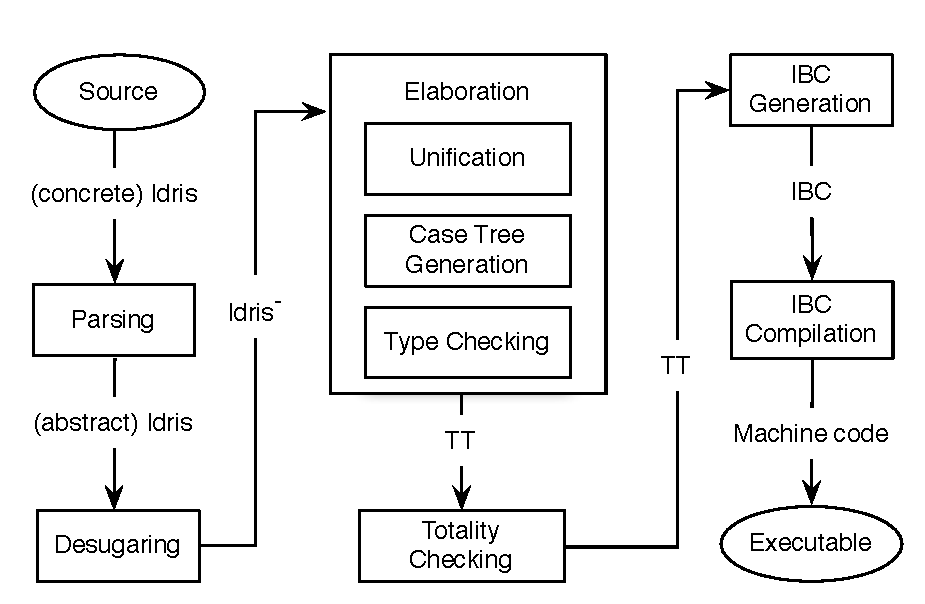
\includegraphics[scale=0.9]{figures/Idris-overview}
\caption{The phases of the Idris compiler. Phases are shown as rectangles, and
  each transition (arrow) is annotated with the input or output representation
  of a given phase. Ovals designate endpoints.}
\label{fig:idris-overview}
\end{figure}
An overview of the different phases of the Idris compiler is shown in
Figure~\ref{fig:idris-overview}. Starting with concrete Idris source code and
ending with a binary executable, each rectangle represents one phase of
compilation. During compilation, the input program is represented in several
different internal languages. Each arrow in Figure~\ref{fig:idris-overview}
is ascribed with the language in which the input program is represented when entering
or leaving a phase, respectively. Omitting a description of the machine code, these are:
\begin{itemize}
\item \textbf{(concrete) Idris}
The high-level language in which Idris programs are written.
\item \textbf{(abstract) Idris}
The abstract representation of the high-level Idris language generated by the parser.
\item \textbf{\IdrisM}
A (strict) subset of abstract Idris without any syntactic sugar. Do-notation and infix operators
are desugared, and implicit arguments are bound explicitly. Note that
\IdrisM{} and abstract Idris are essentially the same language, where the
syntactic sugar from abstract Idris is reduced to desugared terms in \IdrisM.
\item \textbf{TT}
The core type theory, TT, is a dependently typed lambda calculus with inductive
families and pattern matching. TT only allows pattern matching on top-level values,
so all \texttt{case}-expressions are converted to top-level pattern matching
during elaboration. In TT, all terms are fully annotated with their types and
all implicit arguments are explicit.
\item \textbf{Raw}
A (raw) representation of TT terms without any type information. This
representation is used for type reconstruction during type checking. As Raw is
internal to the type checking phase, it is not shown in
Figure~\ref{fig:idris-overview}, but has been included here for completeness and
later reference.
\item \textbf{IBC}
Idris Byte Code (IBC) is the bytecode representation of an Idris program.
\end{itemize}

Each of the language representations (except concrete Idris) are generated by a specific phase of
compilation, usually to reduce a complex representation to a simpler
representation which is easier to reason about and compile. Including the input
and output of the compiler, namely Source and Executable, the phases are:

\begin{itemize}
\item \textbf{Source}
The source code of the program, given in concrete Idris syntax.
\item \textbf{Parsing}
The parser generates an abstract syntax tree (abstract Idris) from the source code.
\item \textbf{Desugaring}
 In the desugaring phase, abstract Idris is reduced to \IdrisM{} by
 desugaring do-notation, implicit arguments, etc.
\item \textbf{Elaboration}
Elaboration reduces \IdrisM{} terms to terms in the core language, TT. The
elaboration phase consists of several notable sub-phases:
\begin{itemize}
\item \textit{Unification} Unification is the process of finding a substitution
  (also called a \texttt{unifier}) that identifies two terms. In Idris,
  unification enables elaboration to progress gradually by continual unification
  of holes with terms, until a complete TT term has been built. Also,
  unification is used for instantiation of implicit arguments. Further details
  will be provided in Section~\ref{sec:elaboration}.
\item \textit{Case Tree Generation}
A case tree\,\citep{Augustsson:1985} is generated for each function definition,
describing the structure of the top-level pattern matching on the left-hand side
of a definition. These case trees are
used for coverage checking by the totality checker.
\item \textit{Type Checking} All TT terms resulting from the previous steps of
  elaboration are type checked at the end of elaboration to ensure that no
  ill-typed terms are constructed. Type checking proceeds by mapping TT terms to
  Raw terms, and then reconstructing the type of each Raw term according to the
  typing environment. If the reconstructed type is convertible with the
  annotated type of the original TT term, type checking succeeds; otherwise, it
  fails. As the last stage of type checking, universe levels are checked by
  checking for cycles in a graph of universe constraints.
\item \textit{Totality Checking} During the totality checking phase, a totality
  analysis is performed on all function definitions. First, a coverage analysis
  determines whether the function in question is covering using the previously
  generated case trees. Next, a termination analysis based on the size-change
  principle is performed on functions with an inductive result type, while a
  productivity analysis is performed on functions with a coinductive result type via the
  syntactic guardedness principle.
\end{itemize}
\item \textbf{IBC Generation}
After successful elaboration, an Idris Byte Code representation is
generated by a script which is built up gradually during elaboration. 
\item \textbf{IBC Compilation}
During compilation, the IBC representation is reduced to machine code.
\item \textbf{Executable}
The final executable generated by the compiler.
\end{itemize}
%\subsection{Internal Representations}
%\subsection{High-Level Abstract Syntax}
%PDecl/PTerm
%	Top level abstract syntax
%	Functions with multiple clauses are multiple Decls

The most interesting parts of the compiler is the core type theory, TT, and the
elaboration phase, in which TT terms are built. These will now be explained in
greater detail. Also, a brief explanation of the implementation of coinductive
data types in Idris will be provided.

\section{TT, the Core Type Theory}
\label{sec:tt-core-type}
\todo{Write a description of how we write TT programs}
% increased confidence
% easier to compile, optimise and type check
%		TT
%			Dependently typed lambda calculus
%			Wrapped in case trees
%			Data and Type constructors??
TT is a dependently typed lambda calculus extended with top-level pattern
matching definitions and inductive families. It is deliberately kept small in order to provide increased
confidence in its correctness. A simple core type theory is also easier to
type check and optimise, and as will be shown in
Chapter~\ref{cha:infer-guard-recurs}, greatly simplifies the implementation of
our inference system for guarded recursion.
\begin{figure}[h]
\centering
\AxiomC{$\Gamma \vdash$ \underline{valid}}
\LeftLabel{Type}
\UnaryInfC{$\Gamma \vdash Type_n : Type_{n+1}$}
\DisplayProof

\vspace{1em}

\AxiomC{$\Gamma \vdash$ \underline{valid}}
\LeftLabel{Const$_1$}
\UnaryInfC{$\Gamma \vdash i : Int$}
\DisplayProof
\quad
\AxiomC{$\Gamma \vdash$ \underline{valid}}
\LeftLabel{Const$_2$}
\UnaryInfC{$\Gamma \vdash str : String$}
\DisplayProof

\vspace{1em}

\AxiomC{$\Gamma \vdash$ \underline{valid}}
\LeftLabel{Const$_3$}
\UnaryInfC{$\Gamma \vdash Int : Type_0$}
\DisplayProof
\quad
\AxiomC{$\Gamma \vdash$ \underline{valid}}
\LeftLabel{Const$_4$}
\UnaryInfC{$\Gamma \vdash String : Type_0$}
\DisplayProof

\vspace{1em}

\AxiomC{$(\lambda x:S) \in \Gamma$}
\LeftLabel{Var$_1$}
\UnaryInfC{$\Gamma \vdash x : S$}
\DisplayProof
\quad
\AxiomC{$(\forall x:S) \in \Gamma$}
\LeftLabel{Var$_2$}
\UnaryInfC{$\Gamma \vdash x : S$}
\DisplayProof
\quad
\AxiomC{$(\underline{let} \mapsto s:S) \in \Gamma$}
\LeftLabel{Val}
\UnaryInfC{$\Gamma \vdash x : S$}
\DisplayProof

\vspace{1em}

\AxiomC{$\Gamma \vdash f : (x : S) \to T$}
\AxiomC{$\Gamma \vdash s : S$}
\LeftLabel{App}
\BinaryInfC{$\Gamma \vdash f\ s : T[{s} / {x}]$}
\DisplayProof

\vspace{1em}

\AxiomC{$\Gamma; \lambda x : S \vdash e : T $}
\AxiomC{$\Gamma \vdash (x : S) \to T : Type_n$}
\LeftLabel{Lam}
\BinaryInfC{$\Gamma \vdash \lambda x : S . e : (x : S) \to T$}
\DisplayProof

\vspace{1em}

\AxiomC{$\Gamma; \forall x : S \vdash T : Type_m$}
\AxiomC{$\Gamma \vdash S : Type_n$}
\LeftLabel{Forall}
\RightLabel{$\exists p.m \leq p, n \leq p$}
\BinaryInfC{$\Gamma \vdash (s : S) \to T : Type_p$}
\DisplayProof

\vspace{1em}

\AxiomC{$\begin{matrix}
\Gamma \vdash e_1 : S
\\
\Gamma \vdash S : Type_n
\end{matrix}$}
\AxiomC{$\begin{matrix}
\Gamma; \underline{let} \x \mapsto e_1 : S \vdash e_2 : T
\\
\Gamma; \underline{let} \x \mapsto e_1 : S \vdash T : Type_n
\end{matrix}$}
\LeftLabel{Let}
\BinaryInfC{$\Gamma \vdash \underline{let}\ x \mapsto e_1 : S.\ e_2 : T[{e_1}/{x}]$}
\DisplayProof

\vspace{1em}

\AxiomC{$\Gamma \vdash x : A$}
\AxiomC{$\Gamma \vdash A' : Type_n$}
\AxiomC{$\Gamma \vdash A \preceq A'$}
\LeftLabel{Conv}
\TrinaryInfC{$\Gamma \vdash x : A'$}
\DisplayProof
\caption{The typing rules for the core type theory TT, borrowed from Brady\,\citep{BradyIdrisImpl13}.}
\label{fig:TT_typing_rules}
\end{figure}
The typing rules for TT are shown in Figure~\ref{fig:TT_typing_rules}. Most of these rules are standard, keeping in mind that types may
depend on values. In order to avoid Girard's paradox, i.e. that the type of
\texttt{Type} is \texttt{Type} (which is a logical inconsistency), a
cumulativity relation ($\preceq$) on universes is used, defined by the rules in
Figure~\ref{fig:TT_cumulativity_relation}.
\begin{figure}
\centering
\AxiomC{$\Gamma \vdash S \simeq T$}
\UnaryInfC{$\Gamma \vdash S \preceq T$}
\DisplayProof
\quad
\AxiomC{}
\UnaryInfC{$\Gamma \vdash Type_n \preceq Type_{n+1}$}
\DisplayProof

\vspace{1em}

\AxiomC{$\Gamma \vdash R \preceq S$}
\AxiomC{$\Gamma \vdash S \preceq T$}
\BinaryInfC{$\Gamma \vdash R \preceq T$}
\DisplayProof

\vspace{1em}

\AxiomC{$\Gamma \vdash S_1 \simeq S_2$} 
\AxiomC{$\Gamma; x : S_1 \vdash T_1 \preceq T_2$}
\BinaryInfC{$\Gamma \vdash \forall x:S_1.T_1 \preceq \forall x:S_2.T_2$}
\DisplayProof
\caption{The rules for the cumulativity relation.}
\label{fig:TT_cumulativity_relation}
\end{figure}
Notice that some of the rules for the cumulativity relation requires terms to be
convertible ($\simeq$), e.g. $S\simeq T$. Convertibility will be explained as
part of the type checking phase in Section~\ref{sec:type-checking}.

The rest of this report will contain both \texttt{TT} and Idris code
examples. Each block of code will be marked indicating what language it
contains. As some details of \texttt{TT} are not necessary to understand our
implementation, we use a different notation for \texttt{TT} than the one used by
Brady\,\citep{BradyIdrisImpl13}. Figure~\ref{fig:tt_notation} shows a \texttt{TT}-function
\texttt{vAdd} as written with first Brady's notation, followed by ours. Firstly,
we treat type class parameters as they are treated in high-level Idris (similar
to Haskell). Secondly we do not annotate the type of pattern variables. Not
shown in the example, we also do not annotate the type of lambda and
let-bindings. Furthermore, we use certain high-level Idris syntactic shorthands, such as
\texttt{[]} instead of \texttt{Nil}. Lastly, note that we use \texttt{=} rather than $\mapsto$.

\newcommand{\lstul}[1]{\ensuremath{\underline{\mbox{ #1}}}}

\begin{figure}[H]
\begin{lstlisting}[mathescape]
vAdd : ($a$ : Type) $\to$ ($n$ : Nat) $\to$ Num $a$ $\to$ 
         Vect $n$ $a$ $\to$ Vect $n$ $a$ $\to$ Vect $n$ $a$
$\lstul{var}$ $a$ : Type, $c$ : Type.
   vAdd $a$ Z $c$ (Nil $a$) (Nil $a$) $\mapsto$ Nil $a$
$\lstul{var}$ $a$ : Type, $k$ : Nat, $c$ : Type,
   $x$ : $a$, $xs$ : Vect $k$ $a$, $y$ : a, $ys$ : Vect $k$ $a$.
   vAdd $a$ (S $k$) $c$ ((::) $a$ $k$ $x$ $xs$)((::) $a$ $k$ $y$ $ys$)
         $\mapsto$ ((::) $a$ $k$ ((+) $c$ $x$ $y$) $xs$) (vAdd $a$ $k$ $c$ $xs$ $ys$)

vAdd : Num a $\Rightarrow$ (a : Type) $\to$ (n : Nat) $\to$ 
         Vect n a $\to$ Vect n a $\to$ Vect n a
vAdd a Z [] [] = []
vAdd a (S k) (x :: xs) (y :: ys)
      = (::) a k (x + y) (vAdd a k xs ys)
\end{lstlisting}  
  \caption{Edwin Brady's\,\citep{BradyIdrisImpl13} notation for \texttt{TT} compared to ours.}
  \label{fig:tt_notation}
\end{figure}

\section{Coinductive Data Types in Idris}
\label{sec:coind-data-types}
Idris supports inductive as well as coinductive type families. The latter is
modeled as lazily evaluated inductive families, where the types of all recursive
constructor arguments are tagged automatically with a special type constructor,
\texttt{Inf}. Values with an \texttt{Inf} type are possibly infinite, and thus
cannot be safely evaluated using a call-by-value strategy. In the vein of Abelson
and Sussman\,\citep{Abelson96SICP}, evaluation of such values is handled by two
special data constructors, \texttt{Delay} and \texttt{Force}. These provide
call-by-name evaluation, in the sense that all \texttt{Inf} values are initally
delayed, and then forced when needed. The compiler cannot always infer all possibly infinite arguments, e.g. when using mixed
induction-coinduction, so in these cases the user must manually tag the correct
argument types with \texttt{Inf}. Aside from the use of \texttt{Inf}, Idris also supports
lazy evaluation of inductively defined values.

\section{Elaboration}
\label{sec:elaboration}
The elaborator is similar to tactic-based theorem provers such as Coq\,\citep{Coq:manual},
which takes terms from \IdrisM{} to TT in a step-by-step manner. The idea is to
construct a TT term from a corresponding \IdrisM{} term by gradual refinement,
until a complete and well-typed TT term has been built. Before describing the
process of elaboration, the motivation behind the elaborator will be provided,
along with the intuitions underlying type checking and totality checking TT terms. 

\subsection{Motivation}
Instead of compiling \IdrisM{} directly to byte code, increased confidence in
the correctness of compilation can be obtained by first transforming a possibly
complex term in the high-level language to a simpler term in the core type
theory. This leads to a smaller trusted core, seeing as if we are
confident that TT can be correctly translated into byte code, and we can
show that any \IdrisM{} term can be correctly transformed
to a corresponding TT term, then we can be more confident in the correctness of
the high-level \IdrisM{} language than if it was translated directly to byte
code.

\subsection{Type Checking}
\label{sec:type-checking}
%Computing normal forms may require evaluation
%The type checker will not attempt to find normal forms for partial definitions.
% Type checking TT terms is a process with two high-level steps:

% \begin{enumerate}
% \item During elaboration, two forms of
% consistency checks are performed, namely type reconstruction and
% conversion checking.
% \item After the TT term resulting from elaboration has been fully built, the
%   definition is \emph{rechecked}.
% \end{enumerate}

% All type checking happens on TT terms. During elaboration, two forms of
% consistency checks are performed, namely type reconstruction and
% conversion checking. A common scenario is as follows:
% \begin{enumerate}
% \item Some tactic expects a term $e$ to have type $A$
% \item The type of $e$ is reconstructed with respect to a context $\Gamma$, such
%   that $e : B$
% \item A conversion check is performed on $A$ and $B$ with respect to $\Gamma$,
%   succeeding if $A$ is convertible with $B$, and failing otherwise.
% \end{enumerate}
% As an example we consider the tactic \textsc{Pi($\Gamma$, $n:S$, $?x:Type.x$)},
% which expects an $x$ of type $Type$, and is given an $n$ of type $S$. The type
% of $S$ is then reconstructed, such that $S : T$. If $T$ is convertible with
% $Type$, then $n$ is a well-typed argument, otherwise it is not.

In the elaboration phase, type checking plays a role both during and after the
construction of a TT term. Type checking a TT term $e$ against a type $T$ is a
twofold process, involving (1) type reconstruction and (2) conversion
checking. To determine whether $e : T$ holds, the type of $e$ is first
reconstructed as $S$, and then a conversion check between $S$ and $T$ is performed.

\subsubsection{Type Reconstruction}
To reconstruct the type of a TT term $e$, all type information is first erased from
the term using a forgetful mapping from TT to Raw, producing $e_{raw}$. The type of the $e_{raw}$ is
then reconstructed such that it conforms to the rules presented in
Figure~\ref{fig:TT_typing_rules}. All type information is available at this
point, so no type inference is performed (no new type information is
derived). Instead, type information is recovered from either the global context,
where the types of top-level definitions are stored, or the local context, where
the types of variables are stored.

\subsubsection{Conversion Checking}
Conversion checking happens by comparing the normal forms of two TT
terms. Finding these normal forms may require evaluation, since any of the two
terms can involve arbitrary expressions. Compile-time evaluation of TT terms is
defined by two contraction schemes, as explained by Brady\,\citep{BradyIdrisImpl13}.
When two TT terms $e_{1}$ and $e_{2}$ are convertible ($\simeq$), such that
$\Gamma\vdash e_{1} \simeq e_{2}$ holds, $e_{2}$ can be
obtained from $e_{1}$ by a finite number of applications of the contraction
schemes, where reversed applications are allowed.

% \paragraph{Aside: Rechecking} When a TT term is returned as the result of
% elaboration, the left-hand side and right-hand sides of a definition are
% \emph{rechecked} against each other using a conversion check, making sure that
% they still match. Rechecking ensures that an elaborated TT term is not only
% well-typed, but actually has the expected type. 

\subsection{Totality checking}
%		Happens during and after elaboration
%			What happens when and why?
%		Coverage: Case Trees
%		Termination: Size Change
%			When are the graphs build?
%		Productivity: Syntactic Guardedness
Totality checking is a prerequisite for type checking, since the conversion
checker will not attempt to find normal forms for definitions which have not
been proven total. In practice, this means that partial functions cannot be part
of a type declaration. The totality
checking procedure in Idris has three parts: coverage checking, totality
checking, and productivity checking.

The coverage checker analyzes the left-hand side pattern matching structure
using case trees\,\citep{Augustsson:1985}. These case trees are constructed from
TT terms by a special case tree elaborator, which in particular identifies
unmatched and default cases. If a definition is not covering, the totality
checker performs no further analysis.

The termination checker is a quite straightforward implementation of the
size-change termination principle\,\citep{LeeJones01SizeChange}. Since Idris
supports the definition of mutually recursive functions in a special block
designated by the keyword \texttt{mutual}, the termination checker
is invoked after the elaboration of each such block.

The productivity checker is an implementation of the principle of
syntactic guardedness\,\citep{Coquand94}. The current implementation is
part of the termination checker, since it merely checks that all
corecursive invocations happen under a special data constructor
``Delay'' (after normalization). The ``Delay'' constructor is used indicate lazy
evaluation, and is eliminated by its counterpart, ``Force''. After normalization,
a corecursive reference must therefore occur under under at least one
``Delay'' constructor in order to be productive.

\subsection{The Elaboration Process}
To enable construction of TT terms by gradual refinement, incomplete terms must
be supported by the elaboration process. Concretely, this happens by having
``holes'' (subgoals of incomplete terms) and ``guesses'' (possible
instantiations for a hole) as binders in the term language, inspired by
McBride's approach\,\citep{McBrideThesis:1999}. Elaboration happens within a
proof state, consisting of the (incomplete) proof term currently being
constructed, a queue of holes, a collection
of unsolved unification problems, and a typing context. At the head of the hole
queue is the hole which is currently being solved. Initially, the proof state
contains only one hole, but more holes can be added to and removed from the hole
queue as elaboration progresses.

As shown in Figure~\ref{fig:idris-overview}, elaboration is a quite complex
process where unification, case tree generation, and type checking are all
intertwined. The invocation of each of these phases is directed by tactics,
since the transformation of different terms requires them at different stages
during elaboration. Elaboration should therefore not be understood as a linear
process from unification to type checking, but rather as a process where each of
these phases are performed as needed.

In practice, elaboration proceeds within a monad \texttt{Elab}, which is
essentially a state monad which also offers error handling and additional
support for specific meta-operations on the state. These meta-operations are
applied to the proof state and the current proof term until all holes have been
resolved. According to Brady\,\citep{BradyIdrisImpl13}, four types of meta-operations are used:
\begin{itemize}
\item \textbf{Queries}, which are the tactics that do not modify the current
  proof term or the proof state. These include retrieving the current proof
  term, retrieving the type of a term, and retrieving the local context of a hole.
\item \textbf{Unification}, which solves unification problems relative to a context.
\item \textbf{Tactics}, which modify the current proof term and may modify the
  proof state in the process.
\item \textbf{Focusing}, which moves a hole to the head of the hole queue.
\end{itemize}
Due to their simplicity, we will forgo explanations of queries and
focusing, an instead elaborate further on unification and tactics.

\subsubsection{Unification}
The goal of unifying two terms $t_{1}$ and $t_{2}$ is to find a substitution
such that the two terms are convertible with respect to a given typing context,
$\Gamma$ (i.e. $\Gamma\vdash t_{1} \simeq t_{2}$). Hence, a unification problem
forms a triple ($\Gamma$, $t_{1}$, $t_{2}$). Unification of two terms may fail
if unification of subterms fail, or if solving one unification problem makes
related unification problems impossible to solve. Solving a unification problem
may lead to solutions of existing problems and introduce new problems.

Unification is used in throughout the elaboration process, for example for type checking
and for the gradual construction of TT terms. Also it is instrumental in the
process of inferring implicit arguments. Consider the implementation of a
\texttt{map} function on indexed lists (\texttt{Vect}) given in
Figure~\ref{fig:vect_map}. Here, \texttt{a}, \texttt{b}, and \texttt{n} are
implicit arguments which must be resolved. First, the implicit arguments are
made explicit through desugaring, as shown in
Figure~\ref{fig:vect_map_desugared}. The types of the implicit arguments cannot
be readily inferred, however, and must be solved by unification. Therefore, the
program in Figure~\ref{fig:vect_map_desugared} gives rise to the following
unification problems:
\begin{itemize}
\item ($\,\cdot\,$, \texttt{a : \_}, \texttt{a : Type})
\item ([a : Type], \texttt{b : \_}, \texttt{b : Type})
\item ([a : Type, b : Type], \texttt{n : \_}, \texttt{n : Nat})
\end{itemize}
The third part of each problem arise from the use of the names: The arguments
\texttt{a}, \texttt{b}, and \texttt{n} are used in positions where
\texttt{Type}, \texttt{Type}, and \texttt{Nat} are expected, respectively. To
solve each problem, the unification algorithm must be able to put a convertible
type at each binding site. In this case, the solutions are all straightforward,
and the resulting program is shown in Figure~\ref{fig:vect_map_resolved}. The
important thing to note is that all of these problems have a unique solution,
making unambiguous inference possible.

\begin{figure}
\begin{lstlisting}[mathescape]
map : (a $\to$ b) $\to$ Vect n a $\to$ Vect n b
map f (x :: xs) = f x :: map f xs
\end{lstlisting}
  \caption{A map function for an indexed list type \texttt{Vect}.}
  \label{fig:vect_map}
\end{figure}

\begin{figure}
\begin{lstlisting}[mathescape]
map : (a : _) $\to$ (b : _) $\to$ (n : _) $\to$ 
      (a $\to$ b) $\to$ Vect n a $\to$ Vect n b
map _ _ _ f (x :: xs) = 
                    ((::) _ _ (f _ _ x) (map _ _ _ f xs))
\end{lstlisting}
  \caption{A desugared map function for a type \texttt{Vect} with implicit
    arguments made explicit.}
  \label{fig:vect_map_desugared}
\end{figure}

\begin{figure}
\begin{lstlisting}[mathescape]
map : (a : Type) $\to$ (b : Type) $\to$ (n : Nat) $\to$ 
      (a $\to$ b) $\to$ Vect n a $\to$ Vect n b
map a b n f (x :: xs) = ((::) n b (f a b x) (map a b n f xs))
\end{lstlisting}
  \caption{A desugared map function for a type \texttt{Vect} with resolved
    implicit arguments.}
  \label{fig:vect_map_resolved}
\end{figure}

\subsubsection{Tactics}
Although unification is an important part of elaboration, the core of the
elaborator is tactics. Tactics modify the current proof term, each describing a
possible step in the transformation of a term from \IdrisM{} to TT. 

%The following are a subset of the tactics which may be part of such a transformation: 

% \begin{itemize}
% \item \textsc{Lambda($\Gamma$, $n$, $?x:T.x$)} creates a lambda binding with
%   respect to a context $\Gamma$ with name $n$, from a proof term which
%   expects a binder ($?x:T.x$).
% \item \textsc{Pi($\Gamma$, $n:S$, $?x:Type.x$)} creates a pi-binding (dependent
%   product type) with name $n$ with respect to a context $\Gamma$, from a
%   proof term which expects a type binder.type checking
% \item \textsc{Let($\Gamma$, $(n:S) \mapsto v$, $?x:T.x$)} creates a let-binding
%   mapping $n$ to $v$ with respect to a context $\Gamma$ from a
%   proof term which expects a binder.
% \item \textsc{Subst($x$, $e$)} which instantiates a hole $x$ with a term
%   $e$, often as a result of unification.
% \item \textsc{PrimUnify($\Gamma$, $e_{1}$, $e_{2}$)} which attempts to unify terms
%   $e_{1}$ and $e_{2}$ with respect to a context $\Gamma$. 
% \item \textsc{Check($\Gamma$, $e$)} which type checks a term $e$ with
%   respect to a context $\Gamma$, returning the type of $e$.
% \item \textsc{Convert($\Gamma$, $e_{1}$, $e_{2}$)} which checks that the
%   cumulativity relation holds between $e_{1}$ and $e_{2}$ by performing a
%   conversion with respect to a context $\Gamma$. 
% \item \textsc{Normalise($\Gamma$, $e$)} which returns the normal form of a term
%   $e$ with respect to a context $\Gamma$.
% \end{itemize}

Tactics describe both concrete operations on the proof term, such as binder
creation, meta-operations on the proof state, such as hole substitution, and
meta-operations ensuring consistency, such as type checking. Complex
operations which require evaluation, e.g. \textsc{Check} and \textsc{Convert},
may invoke operations which are external to the tactic system, such as type
checking.

\subsection{Delaboration}
Mainly to support error reporting, a \emph{de}laborator is also a part of the
compiler. The delaborator builds an \IdrisM{} term from a TT term, striving to
build a term which resembles the user-written term as closely as
possible. However, the delaboration process is not always able to correctly
reconstruct the user-written program, and should therefore not be relied upon
for program analysis.

\section{A Short Recapitulation}
%\todo{Er lidt usikker på denne afslutning, men ellers slutter det næsten for
%brat?}
From the Idris input provided by the user, an abstract syntax tree in abstract
Idris is created. Through desugaring of do-notation and implicit arguments, an
\IdrisM{} representation is built. Elaboration builds a TT term from an
\IdrisM{} term by constructing a proof of a transformation from \IdrisM{} to
TT. This proof is provided as a series of tactics operating on a proof state,
each of which may require unification and type checking. Unification is used for
type checking, term construction, and inference of implicit arguments. Type
checking ensures consistency through type reconstruction and conversion
checks. After elaboration, the totality checker provides the guarantees
necessary for avoiding the reduction of partial definitions during following
invocations of the type checker. During elaboration, a script is accumulated
which describes the resulting IBC file. After the previous phases have been
completed, an IBC file is written, and from this, machine code is generated.

%incomplete terms must be supported by the elaboration process. 


%########
%% TT
% Alt er eksplicit
% Typeregler

%%% Type checking

%% Idris- / Desugaring
% Desugaring er en transformation fra Idris- til Idris-

%% Elaboration
% Hvorfor elaboration?
% Faser "smelter sammen" 
% Teknisk forklaring (tactic prover)

%% Totality checking
% Size-change termination
% Nuværende implementation af produktivitetschecker
% Totality er en forudsætning for type checking
% Erasure? (måske)


%########

%%% Local Variables:
%%% mode: latex
%%% TeX-master: "../copatterns-thesis"
%%% End:


%!TEX root = ../copatterns-thesis.tex
\chapter{Adding Copatterns}
\label{sec:adding_copatterns}
Copatterns can be added to Idris without changing its core, the TT
calculus. Throughout this chapter, we will show how copatterns can be implemented as
syntactic sugar, i.e. a transformation from \IdrisM{} to \IdrisM{}, such that
all copattern clauses have been reduced to pattern clauses by the
time elaboration is reached.

% What, Why
\section{Intuition}
%#########
% Eliminationsregler => Introduktionsregler
% Top-level produktstruktur (een introduktionsregel)
% Pattern matching?
%#########
Following the discussion in Section~\ref{sec:prod-vs.-copr}, support for
copatterns have only been added for record types, both inductive and
coinductive. This decision is based upon the fact that Idris record types have
an obvious top-level structure, making them ideal companions for
copatterns. All examples are therefore given for record types only.

\subsection{The Duality Between Construction and Observation}
\label{sec:dual-betw-constr}
Desugaring copattern clauses, which give definitions by observation, to pattern
clauses, which give definitions by construction, relies on the duality between
introduction and elimination rules for (co)inductive types. For our first example,
we will consider the simple record type \texttt{Pair} in
Figure~\ref{fig:record_pair}. 
\begin{figure}
\begin{lstlisting}[mathescape]
record Pair (a : Type) (b : Type) where
  MkPair : (fst : a) $\to$ (snd : b) $\to$ Pair a b
\end{lstlisting}
  \centering
  $\begin{matrix} 
    \frac { \Gamma \,\vdash\, x\,:\,a \quad \Gamma \,\vdash\, y\,:\,b }{
      \Gamma\, \vdash\,MkPair\,x\,y\,:\,Pair\,a\,b} \scriptstyle I_{Pair}
  & \frac { \Gamma \,\vdash\, e\,:\,Pair\, a\,b }{ \Gamma\,
    \vdash\,fst(e)\,:\,a} \scriptstyle E_{fst}
  & \frac { \Gamma\, \vdash\, e\,:\,Pair\, a\,b }{ \Gamma\, \vdash\,
    snd(e)\,:\,b } \scriptstyle E_{snd}  \end{matrix}$
  $\vspace{12pt}$
  $\begin{matrix}
      \frac { \Gamma\, \vdash\, MkPair\,x\,y\,:\,Pair\,a\,b }{ \Gamma
      \,\vdash\, fst(MkPair\,x\,y)\,\equiv\,x  } \eta_{fst}  & \frac { \Gamma\, \vdash\,
      MkPair\,x\,y\,:\,Pair\,a\,b }{ \Gamma\, \vdash \,snd(MkPair\,x\,y)\,\equiv\,y } \eta_{snd} \end{matrix}$
  \caption{A record defining a type \texttt{Pair}, along with its introduction,
    elimination, and $\eta$-rules.}
  \label{fig:record_pair}
\end{figure}
The traditional way of creating a value of type \texttt{Pair} is by construction
using pattern clauses, as shown in Figure~\ref{fig:pair_example_pattern}. Here,
we construct a value of \texttt{Pair} using its introduction rule, giving the values
\texttt{``Idris''} and \texttt{42} as arguments. We can observe the data in the
constructed value by using the elimination rules \texttt{fst} and \texttt{snd},
which have corresponding $\eta$-rules as expected (see
Figure~\ref{fig:record_pair}). As seen from
Figure~\ref{fig:pair_example_pattern_typing_derivation}, such observations
provide unsurprising results.
\begin{figure}
\begin{lstlisting}
pattern : Pair String Nat
pattern = MkPair "Idris" 42
\end{lstlisting}
  \caption{A value of \texttt{Pair} defined by construction.}
  \label{fig:pair_example_pattern}
\end{figure}

\begin{figure}
\centering
    $
     \frac { \Gamma \,\vdash\, "Idris"\,:\,String \quad \Gamma \,\vdash\, 42\,:\,Nat }{
      \Gamma\, \vdash\,MkPair\,"Idris"\,42\,:\,Pair\,String\,Nat} \scriptstyle
    I_{Pair}$
   $\vspace{10pt}$
  $\begin{matrix} \frac { \Gamma \,\vdash\,MkPair\,"Idris"\,42\,:\,Pair\, String\,Nat }{ \Gamma\,
    \vdash\,fst(MkPair\,"Idris"\,42)\,:\,String} \scriptstyle E_{fst}
  & \frac { \Gamma\, \vdash\,MkPair\,"Idris"\,42\,:\,Pair\,String\,Nat }{ \Gamma\, \vdash\,
    snd(MkPair\,"Idris"\,42)\,:\,Nat } \scriptstyle E_{snd}  \end{matrix}$
   $\vspace{10pt}$
  $\begin{matrix}
      \frac { \Gamma\, \vdash\, MkPair\,"Idris"\,42\,:\,Pair\,String\,Nat }{ \Gamma
      \,\vdash\, fst(MkPair\,"Idris"\,42)\,\equiv\,"Idris"  } \eta_{fst}  & \frac { \Gamma\, \vdash\,
      MkPair\,"Idris"\,42\,:\,Pair\,String\,Nat }{ \Gamma\, \vdash \,snd(MkPair\,"Idris"\,42)\,\equiv\,42 } \eta_{snd} \end{matrix}$
  \caption{Using the rules for \texttt{Pair} on the example in Figure~\ref{fig:pair_example_pattern}.}
  \label{fig:pair_example_pattern_typing_derivation}
\end{figure}

The idea behind copatterns is that we can treat the (co)data constructor as a
black box (\texttt{MkPair} in above example),
defining only the values we expect to observe when making specific observations
on the constructed (co)data. As an example,
Figure~\ref{fig:pair_example_copatterns} shows how we can use copatterns to
define a program by observation which is equivalent to the definition by
construction in Figure~\ref{fig:pair_example_pattern}. The most striking
difference is that \texttt{pattern$^\prime$} itself is never explicitly
defined. Instead, it is defined implicitly by the two copattern clauses, which
provide all the data necessary to derive a corresponding pattern clause, as in Figure~\ref{fig:pair_example_pattern}. From
this observation, we arrive at the main intuition behind our desugaring
procedure: Any definition given by copattern clauses has an equivalent
definition given by pattern clauses, and this definition can be derived without
providing any further information. To make this intuition concrete, consider the
derivation in
Figure~\ref{fig:pair_elimination_on_introduction_rules_rewrite}. Rewriting with
the reduction rules defined in Figure~\ref{fig:pair_example_copatterns}, the
elimination rules for \texttt{Pair} are used to directly derive the right-hand
side of the \texttt{pattern} example from
Figure~\ref{fig:pair_example_pattern}. 

\begin{figure}
\begin{lstlisting}[mathescape]
pattern$^\prime$ : Pair String Nat
fst pattern$^\prime$ = "Idris"
snd pattern$^\prime$ = 42
\end{lstlisting}
  \caption{A value of \texttt{Pair} defined by construction.}
  \label{fig:pair_example_copatterns}
\end{figure}

\begin{figure}
  \centering
$\frac { \begin{matrix} \frac { \Gamma \, \vdash \,pattern'\, :\,
      Pair\, String\, Nat }{ \Gamma \, \vdash \, "Idris"\,:\,String
    } \scriptstyle E_{fst}   & \frac { \Gamma \, \vdash \,pattern'\, :\, Pair\, String\,
      Nat }{ \Gamma \, \vdash \, 42\,:\,Nat } \scriptstyle E_{snd}  \end{matrix} }{
  \Gamma \, \vdash \, MkPair\, "Idris"\, 42\, :\, Pair\, String\, Nat } \scriptstyle I_{ Pair }$
  \caption{Deriving the right-hand side of \texttt{pattern} from \texttt{pattern'}.}
  \label{fig:pair_elimination_on_introduction_rules_rewrite}
\end{figure}

\subsection{Desugaring Copatterns}
While the derivation in
Figure~\ref{fig:pair_elimination_on_introduction_rules_rewrite} provides a fine
display of our intention, such a direct derivation is only possible for simple
examples which have only one resulting pattern clause. In particular, desugaring
copatterns becomes more complex as the following challenges must be taken into account:

\begin{enumerate}
\item Nested copatterns
\item Pattern matching
\item Subsumed copattern clauses
\item Non-covering definitions
\end{enumerate}

To address each of these challenges, we have devised a desugaring procedure for
copatterns which operates in three steps:

\begin{enumerate}
\item \textbf{Expansion}, in which right-hand sides are expanded into partially
  defined constructor invocations.
\item \textbf{Reduction}, in which copatterns are eliminated from the reduction rules.
\item \textbf{Merging}, in which compatible clauses are merged into one clause.
  \begin{enumerate}
  \item Identify compatible clauses
  \item Merge compatible clauses
  \end{enumerate}
\end{enumerate}

Before discussing how our solution tackles each of the challenges, the inner
workings of the procedure will be illustrated with a simple example. Consider
the program \texttt{zeros} in Figure~\ref{fig:zeros}, which produces a value of
the type \texttt{Stream} defined in Figure~\ref{fig:corecord_stream}. In the
first step of desugaring \texttt{zeros}, expansion, the right-hand side of each
copattern clause is expanded into an explicit projection on a partially defined
Stream. Thus, the \texttt{head} clause of Figure~\ref{fig:desugared_zeros_step1}
may be read as: ``The \texttt{head} of \texttt{zeros} is the \texttt{head} of
the partially defined \texttt{Stream} which has \texttt{Z} as its first
constructor argument''. A corresponding reading exists for the \texttt{tail}
clause. \IdrisM{} metavariables are inserted for constructor arguments where
output has yet to be defined, e.g. \texttt{?zeroshead}.

\begin{figure}
\begin{lstlisting}[mathescape]
corecord Stream (a : Type) where
  head : a
  tail : Stream a
  constructor (::)
\end{lstlisting}
  \centering
  $\begin{matrix} 
    \frac { \Gamma \,\vdash\, x\,:\,a \quad \Gamma \,\vdash\, xs\,:\,Stream\,a }{
      \Gamma\, \vdash\,(x\,::\,xs)\,:\,Stream \,a} \scriptstyle I_{Stream}
  & \frac { \Gamma \,\vdash\, s\,:\,Stream\, a }{ \Gamma\,
    \vdash\,head(s)\,:\,a} \scriptstyle E_{head}
  & \frac { \Gamma\, \vdash\, s\,:\,Stream\, a }{ \Gamma\, \vdash\,
    tail(s)\,:\,Stream\, a } \scriptstyle E_{tail}  \end{matrix}$
  $\vspace{10pt}$
  $\begin{matrix}
      \frac { \Gamma\, \vdash\, (x\,::\,xs\,:\,Stream\,a }{ \Gamma
      \,\vdash\, head(x\,::\,xs)\,\equiv\,x  } \eta_{head}  & \frac { \Gamma\, \vdash\,
      (x\,::\,xs)\,:\,Stream\,a }{ \Gamma\, \vdash \,tail(x\,::\,xs)\,\equiv\,xs } \eta_{tail} \end{matrix}$
  \caption{A coinductive record type \texttt{Stream} defining an infinite list,
    along with introduction, elimination, and $\eta$-rules.}
  \label{fig:corecord_stream}
\end{figure}

\begin{figure}
\begin{lstlisting}[mathescape]
zeros : Stream Nat
head zeros = Z
tail zeros = zeros
\end{lstlisting}
  \caption{A function \texttt{zeros} defining a stream of 0.}
  \label{fig:zeros}
\end{figure}

In the second step, reduction, each clause from
Figure~\ref{fig:desugared_zeros_step1} is reduced by removing equivalent
projections on both side of a clause, similar to how one would reduce a
mathematical equation. The result of the reduction is shown in
Figure~\ref{fig:desugared_zeros_step2}. We are allowed to perform such
reductions at this point because all the clauses make right-hand side
projections directly on the (as yet unmerged) output of the function, while all
the left-hand side projections happen directly on the input.

\begin{figure}
\begin{lstlisting}[mathescape]
zeros : Stream Nat
head zeros = head (Z :: ?zerostail)
tail zeros = tail (?zeroshead :: zeros)
\end{lstlisting}
  \caption{Desugaring \texttt{zeros}, step 1: Expansion.}
  \label{fig:desugared_zeros_step1}
\end{figure}

\begin{figure}
\begin{lstlisting}[mathescape]
zeros : Stream Nat
-- Before: head zeros = head (Z :: ?zerostail)
-- Eliminate 'head' on each side
zeros = Z :: ?zerostail
-- Before: tail zeros = tail (?zeroshead :: zeros)
-- Eliminate 'tail' on each side
zeros = ?zeroshead :: zeros
\end{lstlisting}
  \caption{Desugaring \texttt{zeros}, step 2: Reduction.}
  \label{fig:desugared_zeros_step2}
\end{figure}

The final step, merging, is actually a two-step process, where compatible clauses are
merged with each other such that their right-hand sides are combined into
possibly complete constructor invocations. Some of the right-hand sides may remain
incomplete after the merging step if the definition we are desugaring is not
covering. In Figure~\ref{fig:desugared_zeros_step3a}, the clauses of
\texttt{zeros} which are compatible with each other are identified. Since
\texttt{zeros} is a simple example, the two clauses are compatible with each
other because their left-hand sides are identical. The clauses are
therefore merged into one clause, as shown in Figure~\ref{fig:desugared_zeros_step3b}.

\begin{figure}
\begin{lstlisting}[mathescape]
zeros : Stream Nat
-- The two clauses are compatible with each other
(1) zeros = Z :: ?zerostail
(2) zeros = ?zeroshead :: zeros
\end{lstlisting}
  \caption{Desugaring \texttt{zeros}, step 3a: Identifying compatible
    clauses. The clauses have been numbered for reference.}
  \label{fig:desugared_zeros_step3a}
\end{figure}

\begin{figure}
\begin{lstlisting}[mathescape]
zeros : Stream Nat
(1,2) zeros = Z :: zeros 
\end{lstlisting}
  \caption{Desugaring \texttt{zeros}, step 3b: Merging compatible clauses. The
    numbers indicate that both of the clauses from
    Figure~\ref{fig:desugared_zeros_step3a} have been merged into one clause.}
  \label{fig:desugared_zeros_step3b}
\end{figure}

\begin{definition}[\textit{Compatibility}]
\label{def:compatibility}
  Compatibility is a reflexive, transitive, and anti-symmetric binary relation
  $C$ on pattern clauses which describes whether the pattern in one pattern
  clause is more general or equally general to the pattern in another pattern
  clause. Let $V$ be a function which, given an argument pattern, returns the set of
  values matched by that pattern. For two pattern clauses
  $a\,p_{1}\,p_{2}\,\cdots\,p_{n}\,=\,rhs_{a}$ and
  $b\,q_{1}\,q_{2}\,\cdots\,q_{n}\,=\,rhs_{b}$ of an $n$-ary function,
  $(a,b)\in C$ if $V(p_{i})\subseteq V(q_{i})$ for $0 < i\le n$. For a nullary
  function, all pattern clauses are trivially compatible.
\end{definition}
% if the set of values
% for each argument $i$ matched by the pattern of $a$, $P_{i}(a)$, is a subset of of the set of
% values for each argument $i$ matched by the pattern of $b$, $P_{i}(b)$ i.e.
% $P_{i}(a)\subseteq P_{i}(b)$ for all $0 < i\le n$. 

\subsubsection{Addressing the Challenges}
The three-step desugaring procedure presented above has been devised as a
unified solution to four main challenges that arise when desugaring is performed
as a transformation from \IdrisM{} to \IdrisM{}. As we go through each of the
challenges, the \texttt{dupNth} program in Figure~\ref{fig:dupNth} will serve as
a running example of the desugaring of a non-trivial definition with copattern
clauses.

\paragraph{Challenge 1: Nested Copatterns}
Copatterns, i.e. left-hand side projections, can be nested arbitrarily as long
as the nesting is well-typed. As described in
Chapter~\ref{cha:coind-records-idris}, definitions with copatterns only behave
as intended when all projection names are unique. Therefore, our solution
assumes that projection names not only indicate semantics, but also argument
positions to the corresponding constructor. To illustrate, consider the
transformation of clause (2) from Figure~\ref{fig:dupNth} to the expanded clause
\texttt{(2)} in Figure~\ref{fig:desugared_dupNth_step1}. Because this clause
defines the \texttt{head} of the \texttt{tail} of the output, the expanded
clause has the right-hand side, \texttt{head~s}, inserted at this position in
the partially defined constructor on the right-hand side of (2) in
Figure~\ref{fig:desugared_dupNth_step1}. The same reasoning holds for the remaining clauses.

In general, nested copatterns are handled in the first two steps, expansion and
reduction. Expansion ensures that the original right-hand sides are inserted
into the correct positions in the expanded constructor invocations, while
reduction eliminates all left-hand side projections through equational
reasoning. A different solution to the problem of handling nested copatterns has
been proposed by Setzer et al.\,\citep{Setzer14Unnesting}, in which auxiliary
functions are created for each level of nested copatterns. This approach will be
described for an alternative solution in Section~\ref{sec:copatterns-implementation-discussion}.

\paragraph{Challenge 2: Pattern Matching}
Whenever the copattern clauses for a definition have different patterns on the
left-hand side, these patterns must be preserved in the desugared version of the
definition. After eliminating copatterns in the reduction step
(Figure~\ref{fig:desugared_dupNth_step2}), preservation of pattern matching is
ensured in the first sub-step of merging
(Figure~\ref{fig:desugared_dupNth_step3a}), where compatible clauses are
identified. In the following sub-step (Figure~\ref{fig:desugared_dupNth_step3b}), only compatible clauses are
merged. Merging only compatible clauses ensures that a clause is only merged
with other clauses which match the same or a more general set of input values. As an example, we will show exactly why clause (2) is compatible
with clause (1) as postulated in
Figure~\ref{fig:desugared_dupNth_step3a}. The proof
proceeds in Figure~\ref{fig:compatibility_proof}. Note that if, in Figure~\ref{fig:compatibility_proof}, $m_{1}$ had been
$S\,m_{1}$ instead, $(2,1)\notin C$ since $V(S\,m_{1}) =
\{\,x\,|\,x\,:\,Nat\,\setminus\{Z\}\}$, and $V(Z)\not\subseteq V(S\,m_{1})$.

\begin{figure}
From
Definition~\ref{def:compatibility}, we must show: $(2,1)\in C$, where (2) and (1) are clauses from
Figure~\ref{fig:desugared_dupNth_step3a}.
\\\\
We consider the left-hand sides of (2) and (1), respectively:\\
$lhs_{(2)} = dupNth\,s_{(2)}\,n_{(2)}\,Z$\\
$lhs_{(1)} = dupNth\,s_{(1)}\,n_{(1)}\,m_{(1)}$\\
\\
For each sub-pattern, we define the set of matching values:\\
$V(s_{2}) = \{\,x\,|\,x\,:\,Stream\,a\}$\\
$V(n_{2}) = \{\,x\,|\,x\,:\,Nat\}$\\
$V(Z) = \{Z\}$\\
$V(s_{1}) = \{\,x\,|\,x\,:\,Stream\,a\}$\\
$V(n_{1}) = \{\,x\,|\,x\,:\,Nat\}$\\
$V(m_{1}) = \{\,x\,|\,x\,:\,Nat\}$\\
\\
Having defined these, the following must hold:
\\
$V(s_{2})\subseteq V(s_{1}) = \{\,x\,|\,x\,:\,Stream\,a\}\subseteq\,\{\,x\,|\,x\,:\,Stream\,a\}\,\qed$\\
$V(n_{2})\subseteq V(n_{1}) =
\{\,x\,|\,x\,:\,Nat\}\subseteq\,\{\,x\,|\,x\,:\,Nat\}\,\qed$\\
$V(Z)\subseteq V(m_{1}) = \{Z\}\subseteq\,\{\,x\,|\,x\,:\,Nat\}\,\qed$\\\\
Consequently, $(2,1)\in C$
  \caption{From Figure~\ref{fig:desugared_dupNth_step3a}, clause (2) is
    compatible with clause (1).}
  \label{fig:compatibility_proof}
\end{figure}


\paragraph{Challenge 3: Subsumed Copattern Clauses}
In addressing Challenge 2, we stated that different left-hand side patterns must
be preserved in the output. Nevertheless, the pattern from clause (1) in
Figure~\ref{fig:desugared_dupNth_step3a} does not occur in the
desugared version of the function in
Figure~\ref{fig:desugared_dupNth_step3b}. Due to the fact that clause (1) is
more general than all the other clauses, it is subsumed by these in the final
output, such that the right-hand side of (1) is a part of the right-hand side of
both the desugared clauses. The set of subsumed copattern clauses for a
definition are exactly the clauses which are compatible with all other clauses.  

\paragraph{Challenge 4: Non-covering Defintions} As Idris allows users to
define functions which are not covering (see
Definition~\ref{def:covering_function}), partial definitions with copatterns
should be possible as well. With our desugaring procedure, the solution to this
challenge is provided ``for free'', since the metavariables which are inserted
during the expansion phase are simply not replaced with any proper definition if
none is given. A non-covering version of the \texttt{dupNth} function is shown
in Figure~\ref{fig:dupNth_partial}, along with its desugared version.

\begin{figure}
\begin{lstlisting}[mathescape]
||| Duplicate every nth element of s, 
||| starting with the mth element.
||| @s the stream
||| @n how often
||| @m where to start
dupNth : Stream a $\to$ Nat $\to$ Nat $\to$ Stream a
(1) head       (dupNth s n m)       = head s
(2) head (tail (dupNth s n Z))      = head s
(3) head (tail (dupNth s n (S m'))) = head (tail s)
(4) tail (tail (dupNth s n Z))      = tail (dupNth s n n)
(5) tail (tail (dupNth s n (S m'))) = 
                              tail (dupNth (tail s) n m')
\end{lstlisting}
  \caption{A function duplicating the nth element of a stream. The numbers have been
  added to each clause for reference, and are not a part of the actual implementation.}
  \label{fig:dupNth}
\end{figure}

\begin{figure}
\begin{lstlisting}[mathescape]
dupNth : Stream a $\to$ Nat $\to$ Nat $\to$ Stream a
(1) head       (dupNth s n m)       =
      head (head s :: ?dupNthtail)
(2) head (tail (dupNth s n Z))      = 
      head (tail (?dupNthhead :: (head s :: ?dupNthtail)))
(3) head (tail (dupNth s n (S m'))) =
      head (tail (?dupNthhead :: 
                 (head (tail s) :: ?dupNthtail)))
(4) tail (tail (dupNth s n Z))      =
      tail (tail (?dupNthhead :: 
                 (?dupNthheadtail :: tail (dupNth s n n))))
(5) tail (tail (dupNth s n (S m'))) =
      tail (tail (?dupNthhead :: 
                 (?dupNthheadtail :: 
                  tail (dupNth (tail s) n m'))))
\end{lstlisting}
  \caption{Desugaring \texttt{dupNth}, step 1: Expansion.}
  \label{fig:desugared_dupNth_step1}
\end{figure}

\begin{figure}
\begin{lstlisting}[mathescape]
dupNth : Stream a $\to$ Nat $\to$ Nat $\to$ Stream a
(1) dupNth s n m       =
      head s :: ?dupNthtail
(2) dupNth s n Z      = 
      ?dupNthhead :: (head s :: ?dupNthtail)
(3) dupNth s n (S m') =
      ?dupNthhead :: (head (tail s) :: ?dupNthtail)
(4) dupNth s n Z      =
      ?dupNthhead :: (?dupNthheadtail :: 
                      tail (dupNth s n n))
(5) dupNth s n (S m') =
      ?dupNthhead :: (?dupNthheadtail :: 
                      tail (dupNth (tail s) n m'))
\end{lstlisting}
  \caption{Desugaring \texttt{dupNth}, step 2: Reduction.}
  \label{fig:desugared_dupNth_step2}
\end{figure}

\begin{figure}
\begin{lstlisting}[mathescape]
dupNth : Stream a $\to$ Nat $\to$ Nat $\to$ Stream a
-- The 'dupNth s n m' clause is compatible with 
-- all of the other clauses.
(1) dupNth s n m = head s :: ?dupNthtail
-- compatible with (1), (2), and (4)
(2) dupNth s n Z      = 
     ?dupNthhead :: (head s :: ?dupNthtail)
-- compatible with (1), (3), and (5)
(3) dupNth s n (S m') =
     ?dupNthhead :: (head (tail s) :: ?dupNthtail)
-- compatible with (1), (2), and (4)
(4) dupNth s n Z      =
     ?dupNthhead :: (?dupNthheadtail :: 
                     tail (dupNth s n n))
-- compatible with (1), (3), and (5)
(5) dupNth s n (S m') =
     ?dupNthhead :: (?dupNthheadtail :: 
                     tail (dupNth (tail s) n m'))
\end{lstlisting}
  \caption{Desugaring \texttt{dupNth}, step 3a: Identifying compatible
    clauses. The clauses have been numbered for reference.}
  \label{fig:desugared_dupNth_step3a}
\end{figure}

\begin{figure}
\begin{lstlisting}[mathescape]
dupNth : Stream a $\to$ Nat $\to$ Nat $\to$ Stream a
(1,2,4) dupNth s n Z = 
          head s :: (head s :: tail (dupNth s n n))
(1,3,5) dupNth s n (S m') = 
          head s :: 
          (head (tail s) :: tail (dupNth (tail s) n m'))
\end{lstlisting}
  \caption{Desugaring \texttt{dupNth}, step 3b: Merging compatible
    clauses. The numbers indicate which of the clauses from
    Figure~\ref{fig:desugared_dupNth_step3a} that have been merged into each clause.}
  \label{fig:desugared_dupNth_step3b}
\end{figure}

\begin{figure}
\begin{lstlisting}[mathescape]
dupNth : Stream a $\to$ Nat $\to$ Nat $\to$ Stream a
head (tail (dupNth s n Z))      = head s
head (tail (dupNth s n (S m'))) = head (tail s)
tail (tail (dupNth s n Z))      = tail (dupNth s n n)
tail (tail (dupNth s n (S m'))) = tail (dupNth (tail s) n m')
\end{lstlisting}
\begin{lstlisting}[mathescape]
dupNth : Stream a $\to$ Nat $\to$ Nat $\to$ Stream a
dupNth s n Z = 
 ?dupNthhead :: (head s :: tail (dupNth s n n))
dupNth s n (S m') = 
 ?dupNthhead1 :: (head (tail s) :: 
                  tail (dupNth (tail s) n m'))
\end{lstlisting}

  \caption{Above: A non-covering version of \texttt{dupNth}, where the \texttt{head}
    clause has been omitted. Below: its desugared version.}
  \label{fig:dupNth_partial}
\end{figure}


% How
\section{Implementing Copatterns in Idris}

%\subsection{Implementing Copatterns}
%#############
% Hvordan foregår desugaring? 
% Hvordan implementeres intuitionen?
%% Hvilke dele af Idris (jf. figur) berører vi?
% Hvorfor desugaring, i modsætning til elaboration? (mere code sharing)
% Hvorfor udvides TT ikke?

% Identifying copatterns
% Pattern matching
% where-blocks
% Parsing?
% with-rule
% Eksempler (simpelt + avanceret)
% Discussion
%############

\subsection{Parsing Copatterns}
\label{sec:parsing-copatterns}
Identifying copatterns in the concrete Idris syntax turns out to be non-trivial,
due to the rather liberal naming scheme. The Idris parser currently identifies
the leftmost ``naked'' name (without any decorations) in a clause to be the name
of a declared function, a rule which can lead to ambiguities when copatterns
come into play. Notably, the situation presented in
Figure~\ref{fig:copatterns_parsing_hell} is allowed, since Idris allows
declarations and definitions to be freely mixed. The problem in this scenario is
that the two \texttt{head zeros} clauses are syntactically identical, but have
completely different semantics: The first occurrence is the definition of the
function \texttt{head}, and is essentially the constant function for \texttt{Z},
while the second occurrence is a copattern clause for \texttt{zeros}, defining
that the \texttt{head} of \texttt{zeros} is \texttt{Z}.
\begin{figure}
\begin{lstlisting}[mathescape]
zeros : Stream Nat
head : Nat $\to$ Nat
head zeros = Z     -- clause for function 'head'
head zeros = Z     -- copattern 'head' for function 'zeros'
tail zeros = zeros -- copattern 'tail' for function 'zeros'
\end{lstlisting}
  \caption{Copatterns can be difficult to parse, due to situations like
    this. The definition of the type \texttt{Stream} can be found in Figure~\ref{fig:corecord_stream}.}
  \label{fig:copatterns_parsing_hell}
\end{figure}

To resolve such ambiguities, our current solution is simply to prefix each
copattern with a special character, such that copatterns are easily
recognized. Using this strategy, the solution to the situation in
Figure~\ref{fig:copatterns_parsing_hell} is given in
Figure~\ref{fig:copatterns_parsing_hell_fixed_ampersand}. The choice of ``\&''
is arbitrary, aside from the fact that more obvious choices, such as ``.'', are
already used for other purposes. Prefixing with a special character (``.'') is also
the solution chosen by Abel and Pientka\,\citep{Abel13Wellfounded}, although
their language is probably not intended for practical use. Seeing as our current
solution introduces syntax which is quite unlike that of other Idris
constructs, alternative approaches to parsing copatterns will be discussed in
Section~\ref{sec:copatterns-implementation-discussion}.

\begin{figure}
\begin{lstlisting}[mathescape]
zeros : Stream Nat
head : Nat $\to$ Nat
head zeros = Z     -- clause for function 'head'
&head zeros = Z     -- copattern 'head' for function 'zeros'
&tail zeros = zeros -- copattern 'tail' for function 'zeros'
\end{lstlisting}
  \caption{Resolving the ambiguity from Figure~\ref{fig:copatterns_parsing_hell}
  by prefixing each copattern with a special character, here '\&'.}
  \label{fig:copatterns_parsing_hell_fixed_ampersand}
\end{figure}

\subsection{Implementing the Desugaring Procedure}
The desugaring procedure is implemented as a transformation from \IdrisM{} terms
to \IdrisM{} terms, in order to allow for as much as code sharing as possible in
the elaboration phase. In terms of Figure~\ref{fig:idris-overview}, copatterns
are desugared in the Desugaring phase. The idea is that if copattern clauses are
reduced to corresponding pattern clauses as early in the compilation process as
possible, the existing elaboration logic for regular pattern clauses can be
reused in its entirety. Early desugaring also has the implication that no
changes to the core of Idris, the TT calculus, are necessary.

\subsubsection{Implementing Expansion, Reduction, and Merging}
A formalization of the three steps of the desugaring procedure is provided in
Figure~\ref{fig:desugaring_formalization}. The \texttt{expand} function uses the
left-hand side projections to guide the expansion. In particular, the indices on
the projections, i.e. the $i$ in $\pi_i$, denotes the argument position at which
the right-hand side ($\rho_i$) must be given to the constructor. Expansion does
not alter left-hand sides, but leaves right-hand sides expanded as
described. The function \texttt{reduce} is quite simple, removing equivalent
projections on both sides of a clause if the projections occur as the leftmost
expressions on both the left-hand and the right-hand side, respectively. Note that since
\texttt{expand} always returns a clause where the projection pattern on both
sides is identical, \texttt{expand} and \texttt{reduce} can be implemented as
one step in practice, if we simply refrain from reapplying the projections to the
output of \texttt{expand}.

The \texttt{merge} function merges the right-hand side of its second argument
into the right-hand side of its first argument, but only if the two input
clauses are compatible. Merging two right-hand sides is a matter of replacing
the metavariables inserted during expansion with proper terms, an operation
implemented in \texttt{merge$^\prime$}.

\subsubsection{Implementing the Compatibility Relation}
The definition of compatibility (see Definition~\ref{def:compatibility})
requires us to make a pairwise comparison of the sets of matched values for the
argument patterns of two pattern clauses. Taking advantage of the fact that the two
argument patterns compared must not only be well-typed, but also have the same
type (since they are in the same argument position), we can implement the compatibility
relation as a term-level comparison on \IdrisM{} terms. Since two argument patterns
can only have a finite number of different forms, it is possible to encode the
compatibility relation in a table, as shown in
Figure~\ref{fig:compatibility_table}. Whenever two clauses are compatible, we may have to perform one or more
substitutions during the merge step to ensure that the right-hand side of a
merged pattern clause does not refer to names which are not in
scope. Concretely, substitution happens with the function \texttt{subst}, called
by \texttt{merge} in Figure~\ref{fig:desugaring_formalization}, where
\texttt{subs} is a collection of substitutions. Necessary substitutions are indicated in
Figure~\ref{fig:compatibility_table} with ``Yes, if subst.'', which means that
the column pattern must be substituted with the row pattern in the right-hand
side of the merged clause. The substitution function \texttt{subst} performs a simple traversal of the
syntax tree for the right-hand side, replacing terms where necessary.

\subsubsection{Handling \texttt{where}-blocks}
When two pattern clauses are merged, their \texttt{where}-blocks must also be
merged into one. As the last step of merging (not shown in
Figure~\ref{fig:desugaring_formalization}), \texttt{where}-blocks are
concatenated, inventing fresh names for definitions where name collisions
occur. As a consequence, the invented name must be substited for the old name on the
merged right-hand side and in the remainder of the where-block involved. 

\begin{figure}
\begin{lstlisting}[mathescape]
--| Expands the right-hand side to make 
--| projections on a constructor definition
expand $\ulcorner$$\pi_i$ (f x) = $\rho_{i}$$\urcorner$ = 
  $\ulcorner$$\pi_i$ (f x) = $\pi_i$ (MkA ?arg$_1$ ?arg$_2$ $\cdots$ $\rho_i$ $\cdots$ ?arg$_n$)$\urcorner$
expand $\ulcorner$$\pi_j$ lhs = $\rho_{j}$$\urcorner$ = 
  $\underline{let}$ $\ulcorner$lhs$^\prime$ = $\rho_{j}^\prime$$\urcorner$ = expand $\ulcorner$lhs = MkA ?arg$_1$ ?arg$_2$ $\cdots$ $\rho_j$ $\cdots$ ?arg$_n$$\urcorner$
  $\underline{in}$ $\ulcorner$$\pi_j$ lhs$^\prime$ = $\pi_j$ $\rho_{j}^\prime$$\urcorner$
expand $\ulcorner$lhs = $\rho$$\urcorner$ = $\ulcorner$lhs = $\rho$$\urcorner$

--| Reduce an expression by removing equal projections 
--| on the left and right-hand sides of a clause
reduce $\ulcorner$$\pi_i$ lhs = $\pi_i$ $\rho$$\urcorner$  = reduce $\ulcorner$lhs = $\rho$$\urcorner$
reduce $\ulcorner$f x = $\rho$$\urcorner$ = $\ulcorner$f x = $\rho$$\urcorner$
reduce _ _ = error -- Trying to reduce non-compatible projections

--| Merges the first clause with the second clause
--| if they are compatible
merge $\ulcorner$lhs$_1$ = $\rho_1$$\urcorner$ $\ulcorner$lhs$_2$ = $\rho_2$$\urcorner$ =
  $\underline{let}$ (isCompatible, subs) = compatible $\ulcorner$lhs$_1$ = $\rho_1$$\urcorner$ $\ulcorner$lhs$_2$ = $\rho_2$$\urcorner$
  $\underline{in}$ $\underline{if}$ isCompatible
     $\underline{then}$ $\underline{let}$ $\ulcorner$$\rho^\prime$$\urcorner$ = merge$^\prime$ $\ulcorner$$\rho_1$$\urcorner$ $\ulcorner$subst $\rho_2$ subs$\urcorner$
         $\underline{in}$ $\ulcorner$lhs$_1$ = $\rho^\prime$$\urcorner$
     $\underline{else}$ $\ulcorner$lhs$_1$ = $\rho_1$$\urcorner$

--| Merges the first constructor with the second
merge$^\prime$ $\ulcorner$MkA e$_{1_1}$ e$_{2_1}$ $\cdots$ ?arg$_{i_1}$ $\cdots$ e$_{n_1}$$\urcorner$
      $\;$$\ulcorner$MkA e$_{1_2}$ e$_{2_2}$ $\cdots$ $\rho_{i_2}$  $\cdots$ e$_{n_2}$$\urcorner$
     =$\;$$\ulcorner$MkA e$_{1_1}$ e$_{2_1}$ $\cdots$ $\rho_{i_2}$ $\cdots$ e$_{n_1}$$\urcorner$
merge$^\prime$ $\ulcorner$MkA e$_{1_1}$ e$_{2_1}$ $\cdots$ $\rho_{i_1}$ $\cdots$ e$_{n_1}$$\urcorner$
      $\;$$\ulcorner$MkA e$_{1_2}$ e$_{2_2}$ $\cdots$ ?arg$_{i_2}$  $\cdots$ e$_{n_2}$$\urcorner$
     =$\;$$\ulcorner$MkA e$_{1_1}$ e$_{2_1}$ $\cdots$ $\rho_{i_1}$ $\cdots$ e$_{n_1}$$\urcorner$
merge$^\prime$ $\ulcorner$MkA e$_{1_1}$ e$_{2_1}$ $\cdots$ $\rho_{i_1}$ $\cdots$ e$_{n_1}$$\urcorner$
      $\;$$\ulcorner$MkA e$_{1_2}$ e$_{2_2}$ $\cdots$ $\rho_{i_2}$  $\cdots$ e$_{n_2}$$\urcorner$
     =$\;$$\ulcorner$MkA e$_{1_1}$ e$_{2_1}$ $\cdots$ $\rho_{i_1}$ $\cdots$ e$_{n_1}$$\urcorner$
merge$^\prime$ $\ulcorner$MkA e$_{1_1}$ e$_{2_1}$ $\cdots$ MkA($\cdots$)$_{i_1}$ $\cdots$ e$_{n_1}$$\urcorner$
      $\;$$\ulcorner$MkA e$_{1_2}$ e$_{2_2}$ $\cdots$ MkA($\cdots$)$_{i_2}$ $\cdots$ e$_{n_2}$$\urcorner$
     =$\;$$\underline{let}$ $\ulcorner$$\rho^\prime$$\urcorner$ = merge$^\prime$$\;$$\ulcorner$MkA($\cdots$)$_{i_1}$ $\urcorner$ $\ulcorner$MkA($\cdots$)$_{i_2}$$\urcorner$
      $\;$$\underline{in}$ $\ulcorner$MkA e$_{1_1}$ e$_{2_1}$ $\cdots$ $\rho^\prime$ $\cdots$ e$_{n_1}$$\urcorner$
merge$^\prime$ $\ulcorner$$\rho_1$$\urcorner$ $\ulcorner$$\rho_2$$\urcorner$ = $\ulcorner$$\rho_1$$\urcorner$
\end{lstlisting}
\caption{High-level formalization of the desugaring procedure for copatterns,
  given in Haskell-like syntax. \IdrisM{} expressions are given in Quine
  brackets, e.g. $\ulcorner e\urcorner$. Expressions with a preceding ``?'' are
  \IdrisM{} metavariables. The constructor name \texttt{MkA} signifies a
  constructor for an arbitrary type A with a top-level product structure, and $\pi_i$ denotes projections,
  i.e. copatterns on left-hand sides and regular record projections on right-hand sides.}
\label{fig:desugaring_formalization}
\end{figure}

\begin{figure}
  
\begin{center}
  \begin{tabular}{ p{3cm} | c || c | c | c | c | }
    \cline{2-6}
    & $C$ & \quine{$y$} & \quine{\_} & \quine{$c^\prime$} & \quine{MkA($y_1\cdots y_n$)} \\ \cline{2-6}\cline{2-6}
    Pattern variable & \quine{$x$} & \begin{tabular}[c]{@{}c@{}}Yes,\\ if subst.\end{tabular} & Yes & No & No\\ \cline{2-6}
    Placeholder & \quine{\_} & Yes & Yes & No & No\\ \cline{2-6}
    Constant& \quine{$c$} & \begin{tabular}[c]{@{}c@{}}Yes,\\ if subst.\end{tabular} & Yes & if $c$ = $c^\prime$ & No \\ \cline{2-6}
    Constructor pattern & \quine{MkA($x_1\cdots x_n$)}
          & \begin{tabular}[c]{@{}c@{}}Yes,\\ if subst.\end{tabular} & Yes & No & if $C$($x_1$,$y_1$)$\cdots$$C$($x_n$,$y_n$)\\
    \cline{2-6}
  \end{tabular}
\end{center}
  \caption{Encoding the compatibility relation, $C$, in a table, describing
    whether two clause arguments given as \IdrisM{} terms can lead to
    compatibility between two clauses. Consider two clauses, $a$ and $b$ for an
    $n$-ary function, where both clauses have $n$ argument patterns on their
    left-hand side. The argument patterns for $a$ are found in the rows, and
    for $b$ in the columns. Further, let $i$ indicate a position in the sequence of
    argument patterns, such that $0 < i \le n$. For two argument patterns, $p_{i_a}$ and $q_{i_b}$,
    where $p_{i_a}$ is the argument pattern in position $i$ for a clause $a$ and $q_{i_b}$
    is the argument pattern in position $i$ for a clause $b$, each cell answers
    the question: ``Does $C$($p_{i_a}$,$q_{i_b}$) hold?'', i.e. ``Is pattern $q_{i_b}$ more general
    or equally general to pattern $p_{i_a}$?''. Possible left-hand side
    constructs not presented in this table are currently not supported for
    definitions with copatterns (see Section~\ref{sec:merg-comp}).}
  \label{fig:compatibility_table}
\end{figure}
\todo{Is the caption for Figure~\ref{fig:compatibility_table} too long?}

% \begin{figure}
% \begin{lstlisting}[mathescape]
% compatible $\ulcorner$lhs$_1$ = $\rho_1$$\urcorner$ $\ulcorner$lhs$_2$ = $\rho_2$$\urcorner$ = compatible$^\prime$ $\ulcorner$lhs$_1$$\urcorner$ $\ulcorner$lhs$_2$$\urcorner$ $[\;]$

% compatible$^\prime$ $\ulcorner$Ref n$\urcorner$ $\ulcorner$Ref n$^\prime$$\urcorner$ subs
%  | isConstructorName n && isConstructorName n$^\prime$ && n == n$^\prime$
%    = subs
%  | isConstructorName n && isConstructorName n$^\prime$ && n != n$^\prime$
%    = $Not\;compatible$
%  | not (isConstructorName n) && isConstructorName n$^\prime$ && n == n$^\prime$
%    = subs




% compatible' :: Context -> PTerm -> PTerm -> [Substitution] -> Maybe [Substitution]
% compatible' ctxt t@(PRef _ n) (PRef _ n') subs =
%   let sub = (n', t)
%   in case (isConName n ctxt, isConName n' ctxt) of
%        (True,  True)  -> if n == n' then return subs else Nothing
%        (True,  False) -> return (sub : subs)
%        (False, True)  -> Nothing
%        (False, False) -> return (if n == n' then subs else sub : subs)
% compatible' _ (PRef _ _) Placeholder subs = return subs
% compatible' _ (PRef _ _) (PApp _ _ _) _ = Nothing
% compatible' ctxt Placeholder (PRef _ n) subs
%  | isConName n ctxt = Nothing
%  | otherwise        = return subs
% compatible' _ Placeholder Placeholder subs = return subs
% compatible' _ Placeholder (PApp _ _ _) _ = Nothing
% compatible' ctxt t@(PApp _ _ _) (PRef _ n) subs
%  | isConName n ctxt = Nothing
%  | otherwise        = return ((n, t) : subs)
% compatible' _ (PApp _ _ _) Placeholder subs = return subs
% compatible' ctxt (PApp _ (PRef _ n) args) (PApp _ (PRef _ n') args') subs
%  | n == n'   = compatibleArgLists ctxt args args' subs
%  | otherwise = Nothing
% compatible' _ _ _ _ = Nothing
% \end{lstlisting}
%   \caption{A formalization of the compatibility relation.}
%   \label{fig:compatibility_formalization}
% \end{figure}

\section{Discussion}
\label{sec:copatterns-implementation-discussion}
% Is this the best approach to desugaring?
% Would a TT-based approach have been better?
% Discuss 'Unnesting of copatterns' approach
% fejlmeddelelser

While our current approach to desugaring copatterns leads to maximum code
sharing in the elaborator, it comes with its own set of challenges. Concretely
limitations exist for the following:

\begin{itemize}
\item Error reporting
\item Disambiguating names
\item Merging and compatibility
\item The \texttt{with}-rule
\end{itemize}

\subsection{Error Reporting}
After a definition with copatterns has been desugared, errors from the remaining
compilation process no longer occur on the definition provided by the user, but on the desugared version. Obviously,
error messages about terms not written by the user are not very helpful. One way
to alleviate this situation would be store information about the original
copattern clauses in the desugared pattern clauses, such that it would be possible to
retrieve which part of a right-hand side that originated from which copattern
clause. Additionally, extending the delaborator \todo{Do we need to describe the
  delaborator somewhere?} to create copattern clauses from
pattern clauses would be necessary to enable the compiler to create error
messages where the user is shown exactly where his or her implementation is faulty.

\subsection{Disambiguating Names}
Because desugaring of copatterns happens prior to elaboration, we cannot
disambiguate names based on type information. The consequence is that if more
than one projection is defined with the same name, the user must fully qualify
the name for each of the copatterns affected at every application-site. Without
additional information, a more advanced disambiguation scheme is not possible.

\subsection{Merging and Compatibility}
\label{sec:merg-comp}
Merging pattern clauses as directed by the compatibility relation (see
Figure~\ref{fig:compatibility_table}) becomes brittle when viewed from a larger
perspective. Each time a new construct which can appear on a left-hand side is
added to \IdrisM{}, the compatibility relation will have to be
updated. Furthermore, some possible left-hand side constructs, such as functions
and $\Sigma$-types, have no obvious reflexive compatibility relation. For
example, the compatibility relation between two function patterns is difficult to
define. Copattern clauses involving these are therefore currently not supported.

\subsection{The \texttt{with}-rule}
The current implementation does not allow users to use the \texttt{with}-rule on
copattern clauses. Due to the merging step, allowing the \texttt{with}-rule on
copattern clauses would require a procedure for merging two
\texttt{with}-rules into one. At the time of writing, we are not aware of any
such procedure.

\subsection{An Alternative Solution}
As a direct translation to pattern clauses exists for any definition with
copattern clauses, elaborating copattern clauses by reusing the existing
elaboration logic for pattern clauses seems like a logical solution at
first. Working at the level of \IdrisM{} gives rise to many limitations, though,
since most of the type information on terms, case trees, and coverage checking
is not available until later in the compilation process, namely during and after
elaboration. We believe that a more robust solution could be achieved by
elaborating copattern clauses separately, i.e. as a direct transformation from
\IdrisM{} to TT, discarding the solution presented
above.

\subsubsection{Parsing and Disambiguating Names}
One benefit of elaborating copattern clauses separately is that it
allows for name disambiguation from type information. The situation shown in
Figure~\ref{fig:copatterns_type_disambiguation} cannot be solved prior to
elaboration, because the type of \texttt{switcher} requires evaluation. The type
of the pattern for \texttt{switcher} changes according to the boolean argument,
and the corresponding copatterns applied to the pattern must therefore be
derived from an evaluated type. In our current implementation, the user is required to fully
qualify the name for each copattern as soon as more than one projection with the
same name is defined, regardless of namespaces.

Another benefit is that copatterns can be identified more
elegantly. As discussed in Section~\ref{sec:parsing-copatterns}, prefixing all
copatterns with a special character is not a satisfactory solution, neither
aesthetically nor in terms of the concrete syntax of the remaining Idris
constructs. If identification of copatterns is delayed until elaboration, the
situation from Figure~\ref{fig:copatterns_parsing_hell} can be resolved by
introducing a per-definition \texttt{copatterns} block, as exemplified in Figure~\ref{fig:copatterns_parsing_hell_fixed_copatterns_block}.
\begin{figure}
\begin{lstlisting}[mathescape]
namespace A
  corecord Stream a where
    head : a
    tail : Stream a
namespace B
  corecord Stream a where
    head : a
    tail : Stream a

switcher : (c : Bool) $\to$ a $\to$ b $\to$ if c
                                    then A.Stream a 
                                    else B.Stream b
copatterns
  head (switcher True  a _) = a
  head (switcher False _ b) = b
  tail (switcher True  a b) = switcher True a b
  tail (switcher False a b) = switcher False a b   
\end{lstlisting}
  \caption{Elaborating copattern clauses separately allows us to solve this
    situation. From top to bottom, the copatterns for \texttt{switcher} are
    identified as: \texttt{A.Stream.head}, \texttt{B.Stream.head},
    \texttt{A.Stream.tail}, and \texttt{B.Stream.tail}.}
  \label{fig:copatterns_type_disambiguation}
\end{figure}

\begin{figure}
\begin{lstlisting}[mathescape]
zeros : Stream Nat
head : Nat $\to$ Nat
head zeros = Z     -- clause for function 'head'
copatterns
  head zeros = Z     -- copattern 'head' for function 'zeros'
  tail zeros = zeros -- copattern 'tail' for function 'zeros'
\end{lstlisting}
  \caption{Resolving the ambiguity from Figure~\ref{fig:copatterns_parsing_hell}
  by placing copattern clauses inside a per-definition \texttt{copatterns} block.}
  \label{fig:copatterns_parsing_hell_fixed_copatterns_block}
\end{figure}


\subsubsection{Elaboration}
Following Setzer et al.\,\citep{Setzer14Unnesting}, the
complex left-hand side structure of the \texttt{dupNth} function from
Figure~\ref{fig:dupNth} can be simplified as in
Figure~\ref{fig:dupNth_unnesting}. This unnested version leaves us with only
simple copatterns, which can trivially be converted to pattern clauses, as
described in Section~\ref{sec:dual-betw-constr}. Figure~\ref{fig:dupNth_unnesting_pattern_clauses} shows the converted
program. Compared to our current implementation, this strategy for simplifying
copatterns has several advantages. First, it eliminates the need for merging
right-hand sides by creating auxiliary functions. At the \IdrisM{} level,
creating auxiliary functions is non-trivial, because computing the types of such
functions may require evaluation. Secondly, the complex compatibility relation
becomes unnecessary, because pattern matching and copatterns are separated, and
all the resulting copatterns are simple. Thirdly, it enables support for the
\texttt{with}-rule on copattern clauses, since clauses using the
\texttt{with}-rule can be separated into distinct functions, as shown in
Figure~\ref{fig:copatterns_with_rule}.

As a final benefit, a separate elaboration eases meaningful error reporting
considerably. Since user-provided constructs are handled directly, pointing the
user to errors in the concrete syntax is possible without having the delaborator
transform pattern clauses to copattern clauses.\todo{Should we have some sort of
conclusion on this chapter?}

\begin{figure}
\begin{lstlisting}[mathescape]
dupNth : Stream a $\to$ Nat $\to$ Nat $\to$ Stream a
copatterns
 head (dupNth s n m) = head s
 tail (dupNth s n m) = dupNth$^\prime$ s n m

dupNth$^\prime$ : Stream a $\to$ Nat $\to$ Nat $\to$ Stream a
dupNth$^\prime$ s n Z = dupNthZ s n
dupNth$^\prime$ s n (S m$^\prime$) = dupNthS s n m$^\prime$

dupNthZ : Stream a $\to$ Nat $\to$ Stream a
copatterns
 head (dupNthZ s n) = head s
 tail (dupNthZ s n) = tail (dupNth s n n)

dupNthS : Stream a $\to$ Nat $\to$ Nat $\to$ Stream a
copatterns
 head (dupNthS s n m$^\prime$) = head (tail s)
 tail (dupNthS s n m$^\prime$) = tail (dupNth (tail s) n m$^\prime$)
\end{lstlisting}
  \caption{Unnesting the \texttt{dupNth} function from Figure~\ref{fig:dupNth}.}
  \label{fig:dupNth_unnesting}
\end{figure}

\begin{figure}
\begin{lstlisting}[mathescape]
dupNth : Stream a $\to$ Nat $\to$ Nat $\to$ Stream a
dupNth s n m = head s :: dupNth$^\prime$ s n m

dupNth$^\prime$ : Stream a $\to$ Nat $\to$ Nat $\to$ Stream a
dupNth$^\prime$ s n Z = dupNthZ s n
dupNth$^\prime$ s n (S m$^\prime$) = dupNthS s n m$^\prime$

dupNthZ : Stream a $\to$ Nat $\to$ Stream a
dupNthZ s n = head s :: tail (dupNth s n n)

dupNthS : Stream a $\to$ Nat $\to$ Nat $\to$ Stream a
dupNthS s n m$^\prime$ = head (tail s) :: tail (dupNth (tail s) n m$^\prime$)
\end{lstlisting}
  
  \caption{Converting the unnested version of \texttt{dupNth} into pattern clauses.}
  \label{fig:dupNth_unnesting_pattern_clauses}
\end{figure}


\begin{figure}
\begin{lstlisting}[mathescape]
filter : (a $\to$ Bool) $\to$ Stream a $\to$ Stream a
head (filter p s) with (filter p (tail s))
  | s$^\prime$ = if p (head s)) then head s else head s$^\prime$
tail (filter p s) = filter p (tail s)
\end{lstlisting}

\begin{lstlisting}[mathescape]
filter : (a $\to$ Bool) $\to$ Stream a $\to$ Stream a
filter p s = headFilter p s :: filter p (tail s)

headFilter : (a $\to$ Bool) $\to$ Stream a $\to$ a
headFilter p s with (filter p (tail s))
  | s$^\prime$ = if p (head s)) then head s else head s$^\prime$
\end{lstlisting}
  \caption{Above: A \texttt{filter} function on \texttt{Stream}s, showcasing the
    combination of copatterns and the \texttt{with}-rule. Below: The reduced
    version.}
\label{fig:copatterns_with_rule}
\end{figure}
%%% Local Variables:
%%% mode: latex
%%% TeX-master: "../copatterns-thesis"
%%% End:


\chapter{Inference of Guarded Recursion}
\label{cha:infer-guard-recurs}

\section{Intuition}
%##########
% Type-directed (undersøg præcis hvad dette betyder) 
% Overgang fra teori til Idris - Hvilke praktiske hensyn tages der?
% Fix-punktet - hvordan forstås det?
% Kun eet ur!
% Kausale og ikke-kausale funktioner
%% Problemet bag: hvorfor er vi nødt til at skelne?
% Eksempel på inferens
%##########

\section{Implementation}
%##########
% To faser: Inferens og check - bør kunne beskrives separat
% Inferens - regler
% Check - regler
% Correctness claim - Hvordan kan vi være sikre på at vi inferer guarded
% recursion?
% Preservation of semantics - Har den infererede term samme semantik som
% input-termen?
% Tensor-regel og parametre
%##########

%%% Local Variables:
%%% mode: latex
%%% TeX-master: "../copatterns-thesis"
%%% End:


\chapter{Evaluation}
\label{cha:evaluation}
\todo{Link back to motivation}
\section{Guarded Recursion}
In Chapter~\ref{cha:infer-guard-recurs} we discussed an inference and checking
system for guarded recursion. In the following we will present the results of
implementing such a system in Idris, including what can now be proven total, but
also what consequences the scoping we have done has had.

Our goal was to add a less restrictive productivity checker to Idris with
guarded recursion. Let us therefore start by looking at what we can now prove
total in Idris, which we could not before. In
Figure~\ref{fig:productivity_table} a list of function (names) along side their
found productivity with different checking methods can be found. See
Appendix~\ref{sec:guarded-recursion-1} for the implementation of the functions.

\begin{figure}[h]
\begin{center}
  \begin{tabular}{| l | c | c |} \hline
    Function & Syntactic Guardedness & Guarded Recursion \\ \hline
    zeros & Productive & Productive \\ \hline
    repeat & Productive & Productive \\ \hline
    map & Productive & Productive \\ \hline
    zipWith & Productive & Productive \\ \hline
    toggle & Productive & Productive \\ \hline
    interleave & Productive & Productive \\ \hline
    nats & Not Productive & Productive \\ \hline
    fib & Not Productive & Productive \\ \hline
    paperfold & Not Productive & Productive \\ \hline
    paperfold' & Not Productive & Not Productive \\ \hline
%    & & \\ \hline
  \end{tabular}
\end{center}
  \caption{Functions and their productivity according to Idris current totality
    checker and according to our guarded recursion checker. The actual programs
    can be found in Appendix~\ref{app:example-programs}. Note that it is
    according to our system implementing guarded recursion, not guarded
    recursion in general.}
  \label{fig:productivity_table}
\end{figure}

\subsection{Examples of inference}
As we saw we have successfully checked functions for productivity by inferring
guarded recursion. Let us therefore inspect the terms we have inferred, such
that we can convince ourself that we have actually inferred guarded
recursion. Consider the simple example \texttt{zeros}:

\begin{lstlisting}[mathescape]
zeros : Stream Nat
zeros = Z :: zeros
\end{lstlisting}

The first thing we do is to find the guarded
recursive type for the function. Here, \texttt{Stream Nat} becomes $\forall
\kappa$\texttt{.Stream}$^\kappa$ \texttt{Nat}. Once this is done we must find a
transformation from \texttt{Z :: zeros} of type \texttt{Stream Nat} to a term of
type $\forall \kappa$\texttt{.Stream}$^\kappa$ \texttt{Nat}:
\[
IE \vdash Z :: zeros : Stream\,Nat\Longrightarrow \,e : \forall \kappa.Stream^\kappa \,Nat
\]
\[
IE = zeros;\, \causal ;\,\phi, (::,\ _g::), (zeros,\, _gzeros);\, \open;\,
\Gamma,Z : Nat,\ zeros : Stream Nat,\,_gzeros : \forallk{Stream} Nat
\]

We now need to infer a term for $e$. Using the rules from \todo{make ref}, we
end up with the following guarded recursive definition:

\begin{lstlisting}[mathescape]
$_g$zeros : $\forall \kappa$.Stream$^\kappa$ Nat
$_g$zeros = Z $_g$:: (Next$^\kappa$ apply $_g$zeros)
\end{lstlisting}

Details on this inference is to be found in
Appendix~\ref{cha:example-inferences}. A more interesting example is
\texttt{nats}: 

\begin{lstlisting}[mathescape]
nats : Stream Nat
nats = Z :: (map S nats)
\end{lstlisting}

We will not go into a lot of details about this inference here as it is a fairly
complex and long procedure, but what is interesting is that we have to infer a
later composition because of the availability of the recursive reference. We end
up having to infer:

\[
IE \vdash map\,S\,nats : Stream\,Nat\Longrightarrow \,e : \later^\kappa_1 Stream^\kappa \,Nat
\]
\[
IE = nats;\, \curvearrowleft ;\,\phi, (::, _g::), (nats, _gnats), (map, _gmap);\, \sqcup;\, \Gamma
\]

\begin{lstlisting}[mathescape]
$_g$nats : $\forall \kappa$.Stream$^\kappa$ Nat
$_g$nats = Z $_g$:: (Next$^\kappa$ ((apply $_g$map) S) $\tensor ^\kappa _1$ (Next$^\kappa$ apply $_g$nats))
\end{lstlisting}

\subsection{Singleton Clock}
\label{sec:singleton-clock}
\todo{rewrite}
\subsection{Modality}
Another simplification we introduced was modality where we said that a function was
either causal or noncausal. These two are, however, not the only options. Consider
for example the function \texttt{semiinterleave} in
Figure~\ref{fig:semiinterleave}. This function is neither causal, as the
quantification does not span the entire type, not noncausal, as there is not a
quantification on each argument.

\begin{figure}[h]
\begin{lstlisting}[mathescape]
semiinterleave : $\forall \kappa$.Stream$^\kappa$ a $\to$ $\forall \kappa$(Stream$^\kappa$ a $\to$ Stream$^\kappa$ a)
semiinterleave s = $\Lambda \kappa.$ semiinterleave'(s)

semiinterleave' : $\forall \kappa$.Stream$^\kappa$ a $\to$ Stream$^\kappa$ a $\to$ Stream$^\kappa$ a
semiinterleave' = pfix(f)

f : ($\forall \kappa$.Stream$^\kappa$ a $\to$ $\later$$^{\kappa}$(Stream$^\kappa$ a $\to$ Stream$^\kappa$ a)) $\to$ 
       $\forall \kappa$.Stream$^\kappa$ a $\to$ Stream$^\kappa$ a $\to$ Stream$^{\kappa}$ a
f g xs s = StreamCons (head xs)
    (Next (StreamCons (head s) 
                      ((g (tail (tail xs))) $\tensor^\kappa$(tail s))))
\end{lstlisting}
\caption{A function interleave a stream with the even indices of another
  stream.}
\label{fig:semiinterleave}
\end{figure}

The programmer is not able to specify this type in our system, and we can
therefore not correctly check its productivity. We do, however, see that there
are many useful functions which fall into one of these two modality catagories,
and that we have to resort to the more contrived examples, such as
\texttt{semiinterleave}, to find functions we cannot define.

\subsection{User written Guarded Recursion}
While the main purpose of our system is to let users utilize guarded recursion,
without actually writing it, to write productive functions, we aimed to design
our system such that it would be possible to write and check guarded
recursion without any inference. To achieve this we decoupled the inference and
the checking algorithm in such a way that programs already defined as guarded
recursion could be send directly to the checker. 

Sadly, there are other considerations to take, and, currently, a user can not
yet write his own guarded recursive definitions. Taking a side the Idris
technical issues, mainly directing the user written guarded recursion to the
checker, a problem is that in Section \todo{check ref}we eliminated the fixed
point operator.

The checking algorithm expects this kind of guarded recursion without a fixed
point, meaning that this is what the user will have to write. This requires the
user to not only have knowledge about guarded recursion, but also of how our
implementation of it works.

% Brugeren kan ikke, endnu skrive sin egen GR
% Singleton clock og modalitet er hovedsageligt for at gøre inference
% nemmere. Måske checkeren kunne være ligeglad? Det kunne gør at man kunne
% skrive vildere GR programmer selv.
%#############
% GR evaluation 
% Hvor godt virker vores løsning til guarded recursion?
% Hvad virker? Hvad virker ikke?
%% Instans funktioner
%% Relaterede funktioner
% Hvad burde virke?
%#############

%%% Local Variables:
%%% mode: latex
%%% TeX-master: "../copatterns-thesis"
%%% End:


%!TEX root = ../copatterns-thesis.tex
\chapter{Related Work}
\label{cha:related-work}

\section{Copatterns}
\label{sec:related_work_copatterns}
\todo{Relate to 'Unnesting of Copatterns' by Setzer et al.}

\section{Size-change Termination}
Since Idris already has a working totality checker using size-change termination\,\citep{BradyIdrisImpl13}, it would be interesting if the size-change principle could be used for determining the productivity of corecursive functions as well. The size-change principle for termination was first proposed for a strict first-order functional language (without loop constructs) by Lee, Jones, and Ben-Amram\,\citep{LeeJones01SizeChange}. The principle essentially states that if infinitely many recursive calls to a function would lead to infinite decrease in some parameter value, then the function must be terminating, since any value of an inductive type must have finite size. This last condition is of particular importance, as the size-change principle cannot in general recognize functions as being terminating if they have parameters that do not exhibit a well-founded order. Lee, Jones, and Ben-Amram present two realizations of the principle, one using automata and one using a call graph. In the graph formulation, termination is determined by identifying any recursive calls (both direct and indirect) through cycles in the call graph, and then constructing a ``size-change graph'' for each of these. The size-change graphs are then used to find out whether infinite descent in some parameter value is present. One of the limitations of this approach is that parameter values must decrease monotonically: Values cannot at any point become structurally larger, even though the total change in size in a call chain would ultimately lead a to a decreasing value. Two examples of size-change terminating functions are shown in Figure~\ref{fig:sizechange_plus_map}. In both examples, the recursive call happens on structurally smaller input.

\begin{figure}
\begin{lstlisting}[mathescape]
plus : Nat $\to$ Nat $\to$ Nat
plus Z      m = m
plus (S n') m = plus n' m

map : (a $\to$ b) $\to$ Vect n a $\to$ Vect n b
map f []        = []
map f (x :: xs) = f x :: map f xs
\end{lstlisting}
\caption{Two size-change terminating functions.}
\label{fig:sizechange_plus_map}
\end{figure}

Since its first-order formulation, the principle has been proven to be applicable to more expressive cases. Jones and Bohr\,\citep{Jones04Untyped} showed that size-change termination can be applied to the untyped lambda calculus using abstract interpretation\,\citep{Jones:1995}. A set of safe size-change graphs for a program is generated by defining evaluation rules without an environment component, thus overapproximating the number of possible values for any given variable. Given these rules, a corresponding overapproximated set of safe size-change graphs is generated for further termination analysis. Note that due to the undecidability of the halting problem, it is impossible in general to compute the exact set of safe size-change graphs for a given function call.

Following the work on the untyped lambda calculus, Sereni and Jones generalized the size-change principle to handle a higher-order functional language with user-defined data types and general recursion\,\citep{Sereni05terminationanalysis,Sereni06Phd}. Here, a termination criterion is presented which works for arbitrary control-flow graphs, and in turn is able to give an approximation of termination for both strict and lazy functional programs. A key point in this work is how different approaches to control-flow and call graph construction may influence the preciseness of the termination analysis.

All of the previously mentioned implementations of the size-change principle can only approximate termination for programs involving data which exhibits some well-founded order. Nevertheless, Avery\,\citep{Avery06} presented a formulation in which it is possible to detect size-change termination for non-well-founded data types --- in particular, this formulation is shown to work for a language with an integer type. Instead of identifying infinite descent using a well-founded partial order on parameter, as proposed by Lee at al., Avery's analysis is based on a decrease in invariants which are found to hold for each program point. The idea is that if the value of some invariant (which can involve arbitrarily many values) can be shown to decrease on every passage of a program point, then the program terminates. A simple example of a size-change terminating program in Avery's implementation is given in Figure~\ref{fig:avery_example}. The invariant for the inner loop is \texttt{n - j + i}, while the one for the outer loop is \texttt{n - i}. These cannot decrease indefinitely, and therefore the program is size-change terminating.

\begin{figure}
\begin{lstlisting}
for (i = 0; i <= n; i++) {
  for (j = 0; j-i <= n; j++);
}
return;
\end{lstlisting}
\caption{An example program involving integers written in a subset of C, which is size-change terminating in Avery's formulation.}
\label{fig:avery_example}
\end{figure}

While size-change termination for non-well-founded data could be a step towards using a size-change approach for an approximation of productivity, it is unclear which invariants one would have to infer for corecursive programs. A first attempt might emerge from the observation that any productive corecursive program cannot consume any more data than it produces. Based solely on syntax, such an analysis would quickly approach the idea behind syntactic guardedness checkers, which will be discussed in Section~\ref{sec:synt-guard}.

In more recent work, Hyvernat\,\citep{Hyvernat13} has proposed a formulation of the size-change principle for functional languages which to a certain degree solves the problem of non-monotonic decrease in parameter values. The motivation behind this work is to incorporate size-change termination into the PML language\,\cite{PMLLanguage}. Non-monotonic decrease is detected by tracking the size of a parameter throughout the entire control-flow graph, instead of merely recording whether each call in isolation leads to a decrease in some value.

The termination criterion most similar to the size-change principle predates the original article by Lee, Jones, and Ben-Amram\,\citep{LeeJones01SizeChange}. This criterion was developed by Abel for the \texttt{foetus} termination checker\,\citep{Abel98foetus}, and forms the basis of the totality checker implemented in Agda\,\citep{Norell:thesis}. Analogous to the size-change principle, Abel identifies recursive calls in a call graph and performs a termination analysis by tracking changes in parameter sizes. This initial presentation of \texttt{foetus} makes no mention of productivity for corecursive programs, although such an extension has since been presented by Altenkirch and Danielsson\,\citep{AltenkirchNAD10} (for further discussion, see Section~\ref{sec:synt-guard}).

\section{Syntactic Guardedness}
\label{sec:synt-guard}
% Telford and Turner nævnes mere
% Hyvernat flyttes herned

Due to the duality between inductive and coinductive types, it may be compelling to imagine a productivity analysis which, dual to the size-change principle, works by identifying structurally larger values. Such a dual notion of ``size-change productivity'' is exactly the idea behind the syntactic guardedness checkers found in Idris, Agda, and Coq\,\citep{Coq:manual}. Where values become structurally smaller by pattern matching, they become structurally larger by constructor application. Therefore, the \emph{guardedness principle} states that a coinductive definition is guarded if all corecursive calls appear directly under a coinductive constructor. This has the implication that the productivity of corecursive functions can be detected by a purely syntactic check.

The guardedness principle was first proposed by Coquand\,\citep{Coquand94} has a tool for constructive reasoning about infinite objects. Coquand argues that previous coinductive proof methods rely on impredicative definitions, which he deems to be ``unsatisfactory'' for constructive reasoning. Based on Milner's work on process calculi\,\citep{Milner:1989}, Coquand defines an infinite object to be productive if a (not necessarily well-founded) computation tree can be associated with it, through an analogy between infinite proof objects and processes. This observation is then synthesized into a ``guarded induction principle''. In practice, the guarded induction principle can be used for constructive proofs through a syntactic check, which verifies that all corecursive references appear directly under a coinductive constructor.

In continuation of Coquand's efforts, Gim\'{e}nez\,\citep{Gimenez95} formalized an extension of the Calculus of Constructions\,\citep{Coquand:1988}, in which a modification of Coquand's original formulation of the guarded induction principle is provided. In particular, the guarded induction principle is modified such that it can be applied to types with second-order quantification.

The guarded induction principle described by Coquand and Gim\'{e}nez was intended to be used within a proof system (e.g. Coq) for easier reasoning about infinite objects. Confirming Coquand's own observation, Telford and Turner\,\citep{Telford98ensuringthe} argue that the guarded induction principle is too conservative in a programming setting. In their system of \emph{Elementary Strong Functional Programming} (ESFP)\,\citep{Telford97ensuringstreams,Telford98ensuringthe,Telford:jucs_6_4:ensuring_termination_in_esfp}, Telford and Turner therefore extend practical use of the guarded induction principle to detect a wider range of function as productive. They achieve this by considering guardedness more abstractly over a domain of ``guardedness levels'', such that productive corecursion is bounded by a given ``depth''. Intuitively, their system works by detecting that a program produces more elements that it consumes, i.e. that recursive references are subject to more introduction forms (constructor applications) than elimination forms (case analysis). Since any program can be higher-order, the guardedness level of a function is calculated by a ``guardedness function'',  where the guardedness levels of both bound and free variables are taken into account. As an advanced example, Telford and Turner show that the program generating the Hamming numbers (a problem first discussed by Dijkstra\,\citep{Dijkstra:1997}) is accepted as a productive program by their system.

Hyvernat\,\citep{Hyvernat13} discusses an approach similar to the idea behind the work of Telford and Turner. He proposes that productivity can be detected by counting the number of abstractions and applications in a program, respectively. Given that one does not reduce under abstractions, a function can then be considered productive if it has more abstractions than applications, since this necessarily means that the program will not diverge.

Another approach to coping with the conservative nature of the original guardedness principle is to consider alternative programming styles, making productive definitions easier to write. Following the incorporation of the guardedness condition into the Agda totality checker as described by Altenkirch and Danielsson (they attribute their approach to Abel)\,\citep{AltenkirchNAD10}, Danielsson\,\citep{Danielsson10beatingthe} described a method for working around the guardedness condition whenever it rejects a productive program. When a corecursive reference appears under a call to a function which is not a constructor, he designs an embedded domain-specific language in which said function is implemented as a constructor, making the guarded induction principle applicable. He is then able to define an interpreter for this language, such that the original program is ultimately accepted as productive. None of these steps happen automatically, but must be done manually. Although useful, Danielsson argues that efficiency is a concern, and that the best solution might be to entirely move away from using guardedness for productivity. Sized types have since been implemented in Agda.

\section{Guarded Recursion}
%Nakano
%neelk
%Atkey and McBride
%Flere papers fra Aarhus + Mogel

As presented in Section~\ref{sec:guarded-recursion}, guarded recursive type systems can be used to define necessarily productive programs. The general notion underlying guarded recursion was introduced by Nakano\,\citep{Nakano:2000}, although he does not himself use the term ``guarded recursion''. He introduces a modal typing system with recursive types, $\lambda\!\bullet\!\mu$, in which it is possible to encode provably non-diverging programs. This is achieved partly by giving a modal type to the Y-combinator (see Figure~\ref{fig:nakano_Y}), and partly by defining types such that recursive occurrences are only available in the context of a modality $\bullet$, e.g. infinite binary trees as a type $\mu X.A\times\bullet X\times\bullet X$. Nakano suggests that his system could be related to temporal logic, where the $\bullet$ modality reprensents notions of ``previous time''. Additionally, he notes that the system is not intended to be used as a type system for programming languages, but serves to widen the range of programs to which the idea of proofs-as-programs can be applied.

\begin{figure}
\[
\vdash \lambda f. (\lambda x. f (x x)) (\lambda x. f (x x)) : (\bullet X \to X) \to X
\]
\caption{The Y-combinator as derived in Nakano's $\lambda\!\bullet\!\mu$ system\,\citep{Nakano:2000}.}
\label{fig:nakano_Y}
\end{figure}

Inspired by Nakano's approach, Atkey and McBride\,\citep{Atkey:2013} present a similar typing discipline based on the simply typed lambda calculus, paving the way for a more practical use of guarded recursion. They introduce applicative programming\,\citep{Mcbride:2008} over modalities, which coupled with Nakano's fixed point combinator makes programming with modalities more accessible, and provides a more compositional system for productivity checking. Their main contribution is the introduction of clock variables into a type system with guarded recursion, such that it is possible to distinguish between values that are in the process of construction and values that are fully constructed. Fully constructed values can be identified by universal quantification over clock variables, enabling the user to extract values from the modal world of guarded recursion.

Following the work by Atkey and McBride, M\o gelberg\,\citep{Mogelberg:2014} extends the idea of a type system with guarded recursion and clock variables to a dependently typed setting. Based on work by Birkedal and M\o gelberg\,\citep{BirkedalL:sgdtuniverse-conf} and Birkedal, M\o gelberg, Schwinghammer, and St\o vring\,\citep{BirkedalL:sgdt-journal}, he models a dependently typed lambda calculus with guarded recursion and clocks using the topos of trees model. This results in an extensional type theory for reasoning about guarded recursive types. Although no intensional formulation of the model is given, it is expected that such a formulation exists.

% In extensional type theory, definitional and propositional equality is the same
Typing systems with modalities on types as introduced by Nakano has also been applied in the field of functional reactive programming. Krishnaswami\,\citep{Krishnaswami13} presents a typing system where both time leaks (depending on past values for arbitrary intervals of time) and space leaks (non-permanent memory leaks from capturing too much history) are prevented by construction. This is accomplished by typing all values with \emph{temporal recursive types}, using modalities on types to indicate the time at which a value becomes available. In the context of a global clock, programs are then evaluated according to two operational semantics: one giving the semantics for a program at the current clock tick, and one for advancing the global clock. Whenever the global clock is advanced, all values which can no longer be referenced due to time constraints are discarded from the environment, thus eliminating space leaks. Accompanying this mechanism are rules which make references to unavailable data impossible. Time leaks are prevented by unfolding all values at the moment they become available. Since Krishnaswami's approach enforces causality (that the first \emph{n} outputs only depend on the first \emph{n} input values), it can essentially be used to encode guarded recursion, at least in the simply typed formulation by Atkey and McBride. But where Atkey and McBride emphasize that clock variables localize the encoding of productivity, Krishnaswami introduces a global clock to which all programs must adhere.

\section{Sized Types}
An alternative approach to type-based totality checking is sized types. Where the intuitive abstraction of guarded recursion is time, sized types attach sizes to values at the type level. The motivation behind sized types is to express totality proofs using induction on sizes, such that the structure of the term in question can be disregarded. With size-change termination, termination proofs are constructed by ensuring that all recursive arguments happen on structurally smaller terms. Analogously, totality proofs using sized types are constructed by ensuring that all values are defined in terms of data with a structurally smaller \emph{size}.  Hence, the term ``size'' implies no specific term structure on the data involved in the totality proof.

Sized types for totality checking were first proposed by Hughes, Pareto, and Sabry\,\citep{Hughes96} for reactive systems, where each data type introduced into a program is associated with a family of sized types indicating the bounds of a value of that type. A similar idea was developed by Amadio and Coupet-Grimal\,\citep{Amadio98}, where guard conditions are introduced into the type system to ensure the productivity of coinductive data, following the work of Coquand\,\citep{Coquand94} and Gim\'{e}nez\,\citep{Gimenez95}.

Eduarde Gim\'{e}nez also presented a system for typing recursive definitions in an extension of the Calculus of Constructions using sized types\,\citep{Gimenez98structuralrecursive}. A notable result of this work is that any well-typed term in the proposed extension is normalizing with respect to lazy evaluation, substantially widening the domain of functions to which type-based termination is applicable. In the wake of this extension, Abel\,\citep{Abel99terminationchecking} wrote a quite accessible paper on using sized types for totality checking, showing that bidirectional type checking\,\citep{Pierce00} is suitable for a system with sized types. In addition, it is described how infinite streams defined as coinductive types can be encoded in a language as functions on natural numbers, and that the productivity of a stream can be understood in terms of its \emph{definedness}, meaning the number of times it can safely be unfolded.

The notion of definedness is also an important part of Abel and Pientka's work on applying sized types to a system with copatterns\,\citep{Abel13Wellfounded}, although here it is defined more precisely as the \emph{depth} of a value of coinductive type. By directly using the notion of depth in the type system, they show that totality proofs for both coinductive definitions with copatterns and inductive definitions (as well as mixed inductive-coinductive definitions) can be constructed by well-founded induction on sizes within the type system. The method is shown to work for System F\textsubscript{$\omega$}, and has later been implemented in Agda along with copatterns.

%structurally smaller

%%% Local Variables:
%%% mode: latex
%%% TeX-master: "../copatterns-thesis"
%%% End:



%!TEX root = ../copatterns-thesis.tex
\chapter{Future Work}
\label{cha:future-work}
In this chapter we will discuss how we see our project evolve in the
future. While we have implemented both copatterns and a new productivity checker
in the Idris compiler, the following sections are characterized by what we have learned
during the development of these. Both of the solutions could be improved
and extended in several different interesting ways. 

% Late in the forming of our solutions, we have discovered better
% solutions than the ones we have implemented. Sadly, our discoveries of better
% approaches have surfaced too late to be implemented for this report. What we see
% as future work is therefore pervaded and inspired by our plans to improve our implementation.
\section{Copatterns}
While our implementation of copatterns does work, there are improvements to be
made. In Section~\ref{sec:copatterns-implementation-discussion} we discussed
several topics, and in the following we will go over those which inspire future work.
\subsection{An Alternative Solution}
While we have implemented copatterns as a desugaring from \IdrisM{} definitions
to \IdrisM{} definitions,
we proposed an alternative implementation in
Section~\ref{sec:an-altern-solut}. This solution moves our implementation from
from a desugaring of \IdrisM{} to an elaboration from \IdrisM{} to
\texttt{TT}. This seems like a more robust solution which simplifies the disambiguation
of names, a problem discussed in Section~\ref{sec:pars-disamb-names}.
\subsection{Improved Syntax}
As a solution based on elaborated copatterns rather than desugaring
simplifies name disambiguation, it also opens up new syntactical options. In
Section~\ref{sec:parsing-copatterns}, we discussed that we are not happy with
prefixing all copatterns with a special character, and therefore suggested a
per-definition \texttt{copatterns} block as an alternative in
Section~\ref{sec:pars-disamb-names}. A simple implementation of such a
\texttt{copatterns} block could already now be implemented by making the parser
more clever, but this is not a desirable solution in general.
\subsection{The \texttt{with}-rule for Copattern Clauses}
In the presence of inductive families, the \texttt{with}-rule is a very powerful
tool, allowing users to match on intermediate calculations. In
Section~\ref{sec:textttwith-rule} we explained how the current copatterns implementation
does not work with the \texttt{with}-rule. As such, an interesting future
improvement is to have copattern clauses compatible with the \texttt{with}-rule in Idris.

%### Copatterns ###
% Copatterns in with-rule
% Pattern matching på codata i Idris?
% Måske bedre syntaks
% 
%##################
\section{Guarded Recursion}
\label{sec:guarded-recursion-1}
The most important continuation of our project is to reintroduce the fixed point
operator into our implementation. In Section~\ref{sec:depend-funct-types} we
discussed the implications of such a reintroduction for the inference and
checking system, respectively. In practice, readjusting our implementation to
work with the fixed point operator would be a simple task. Having the fixed
point operator means that all rules for recursive references could be replaced
by one, simple rule. Additionally, this would simplify a working implementation
with support for non-causal functions.

Our intention is to implement a system without fixed point elimination within a reasonable
time frame. Therefore, we will base our suggestions for future work on a new, improved
implementation.

% \subsection{General Improvements}
% We have previously discussed totality dependencies, in
% Section~\ref{sec:total-depend}, and general bugs in our implementation, in
% Section~\ref{sec:our-implementation}. We intend to implement and fix these
% problems alongside a implementation of the fixed point operator.

\subsection{Type Class Instances}
Our implementation does not currently work for type class instances in
Idris. This is not an
inherent flaw of our system, but rather because our implementation does not
treat type classes in any special way.

In Section~\ref{sec:type-class-instances} we briefly touched upon a possible
solution to this problem. For any coinductive type, we not only infer a
guarded type, but we also infer its guarded instances. As an example, we
consider \texttt{Stream} as an instance of the type class \texttt{Functor}:

\begin{lstlisting}[mathescape, title=\idrisBlock]
instance Functor Stream where
  map f (x :: xs) = (f x) :: (map f xs)
\end{lstlisting}

To use the guarded stream, \texttt{Stream}$^\kappa$, as a \texttt{Functor} as well, we
must infer an instance of \texttt{Functor} for \texttt{Stream}$^\kappa$. We do
this by creating a new instance \texttt{Functor Stream}$^\kappa$, and use our
inference system to infer a guarded term for the implementation:

\begin{lstlisting}[mathescape, title=\idrisBlock]
instance Functor Stream$^\kappa$ where
  map f (x $_g$:: xs) = (f x) $_g$:: (Next$^\kappa$ (map f) $\tensorkappan$ xs)
\end{lstlisting}

% Implementing this, while seemingly simple, could be complicated as it requires a
% thorough understanding of type classes in Idris. Both how they are elaborated to
% TT, and how they behave in TT. The main task of adding type
% classes to our implementation is therefore understanding type classes in Idris.

\subsection{Mutual Recursion}
We discussed how we are unable to ensure productivity for mutually recursive
functions, as our analysis prevents infinite recursion by securing that the
recursive reference is only available later. Because mutual recursion can lead
to infinite recursion through other constructs, we can not prove any mutually
defined function definitions productive.

Clouston et al.\,\citep{BirkedalL:guarded-lambda-conf} discuss that one solution
to mutual recursion is to define the fixed point for a product of functions. A
similar approach could be adopted in our system to support mutual
recursion. This would require changes to the inference system, because since it
would have to take more than one recursive reference into account. No changes
would be needed in the checking system, as the fixed point rule works for elements any
(non-dependent) type, and thereby also for a product of functions.

\subsection{User-written Guarded Recursion}
Another interesting continuation of our project is to allow user-written
guarded recursion. In Section~\ref{sec:user-written-guarded}, we discussed the
challenge of allowing the user to write guarded recursion, namely that arbitrary
axioms could be added to the checking system by allowing pattern matching on
values of type $\laterkappa$A. 

% In order to allow user-written guarded recursion
% to exist alongside our inference system, further research Are there other such pitfalls to avoid, or can we simply
% just disallow pattern matching on \texttt{Later} types?

A first step towards user-written guarded recursion in Idris could be to
allow the user to specify guarded recursive types, but still let the system infer the
guarded recursive term. We already let the user specify part of the type, namely
whether it is causal or non-causal. By allowing the user to fully specify the guarded type, we could get
closer to checking productivity of such functions as those described in Section~\ref{sec:function-types}.

\subsection{Multiple Clocks}
We restricted our system to a singleton clock environment to simplify
inference. However, in Section~\ref{sec:multiple-clocks} we argued that
extending the type checker to multiple clocks could work well alongside
user-written guarded recursion. This would not affect the inference system, as
it would still not infer definitions with multiple clocks. 

\subsection{Dependent Types and Guarded Recursion}
In Section~\ref{sec:handling-parameters} we discussed the problems of type
substitution when using later application, and how it has affected our
system. Should future research show that type substitution is indeed sound for
later application, adjusting our system would be straightforward, yet
important. Should the rule from Figure~\ref{fig:tensor_with_subst} prove to be
sound, it would change the $\infer_{\tensorkappan}$-rule and the
$I_{\tensorkappan}$-rule as shown in
Figure~\ref{fig:tensor-rules_with_type_subst}. As such, it is possible to adjust
our system to at least some possible further research in the area of guarded recursion and
dependent types.

\begin{figure}[h]
\centering

\AXD{\begin{matrix} \IEopen \, \vdash \, f\, :\, (a' : A)\, \to \, B\, \infer \,
    g\,:\, \laterkappan ((a : A')\, \to \, B') \\ 
                    \IEopen \, \vdash \, x\, :\, A\, \infer \, y\,:\,\laterkappan A'
     \end{matrix}} 
\RLabel{n \geq 1, f \not = \iota \quad (\infer_{\tensor^{\kappa}_{n}})} 
\UID{\IEopen \, \vdash \, f\, x\, :\, B[{x}/{a}]\, \infer \, g\, \tensor^{\kappa}_{n} \, y\, :\, \laterkappan B'[{y}/{a'}]}
\DisplayProof
  
\vspace{1em}

    \AxiomC{$\CEopen \vdash t : \laterkappan ((a : A) \to B) $}
    \AxiomC{$\CEopen \vdash u : \laterkappan A$}
    \RightLabel{$I_{\tensorkappan}$}    
    \BinaryInfC{$\CEopen \vdash t \tensorkappan u : \laterkappan B[{u}/{a}]$}
\DisplayProof  
  \caption{$\infer_{\tensorkappan}$ and $I_{\tensorkappan}$ rules with type
    substitution.}
  \label{fig:tensor-rules_with_type_subst}
\end{figure}

%%% Local Variables:
%%% mode: latex
%%% TeX-master: "../copatterns-thesis"
%%% End:


%!TEX root = ../copatterns-thesis.tex
\chapter{Conclusion}

\bibliography{bibliography}

\end{document}

%%% Local Variables: 
%%% mode: latex
%%% TeX-master: t
%%% End: 
